\chapter{Introduction to \SB{} and \cocos{} }
Now it's time to dive into 2D Game Development! For this chapter I will assume
that you haven't written a game with a game engine yet. We will be discussing
all the relevant concepts throughout this chapter.

\section{Installing the software}
First things first. Let's install the software used throughout this book.
In general there are two ways to install \cocos{} depending on whether you want
to use \SB{} or not. In this book we will be using \SB{} to set up all
of our projects, therefore we will only install \SB{} which will come bundled
with the latest version of \cocos{}. 

Installing \SB{} is easy, simply open the \textit{App Store} app on your Mac and
search for \textit{SpriteBuilder}. Note that you should always use the latest
version of Mac OS X and \xcode{} together with \SB{} (as of this writing Mac
OS X 10.9 and \xcode{} 6.0).

\begin{figure}[H] 
		\centering
		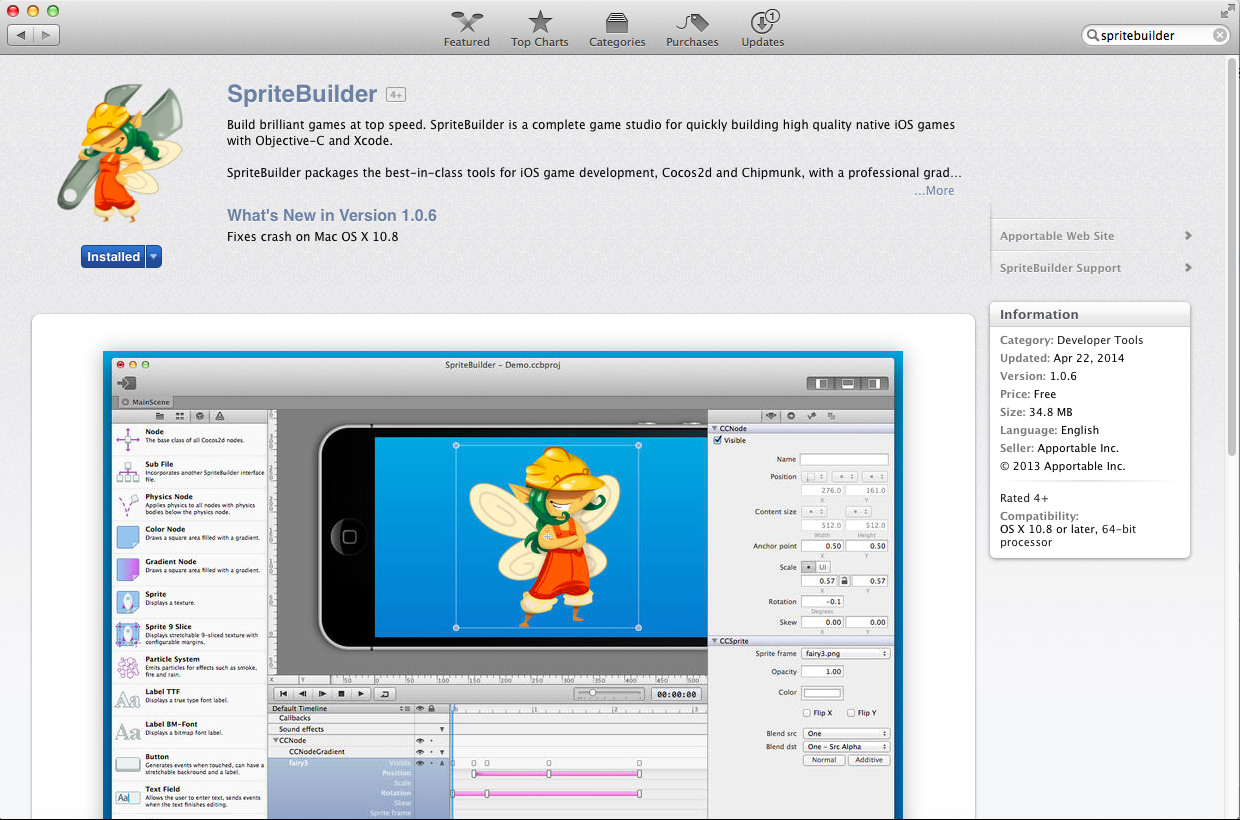
\includegraphics[width=200pt]{images/cocos2d/setup/mac_appstore_install.png}     
		\caption{\cocos{} Technology Stack}
\end{figure}

After a couple of minutes the \SB{} installation should be completed. Later
throughout this chapter you will learn how to set up your first project.

\section{Why \cocos{}}
Well, now you have already installed \cocos{}. I still want to spend a moment on
discussing why we are using this tool. The main goal of \cocos{} is to make
mobile game development \textit{easier}. Earlier we have discussed the basic
concepts and benefits of game engines. You should now know that there are many
problems developers have faced while developing games, animations, physics, etc.
- and most of them have been solved and put into frameworks. You should not
spend your precious time trying to solve them again. So now that you know that
you definitely should use a framework - \textbf{which ones are available and why
should you choose \cocos{}}?

\textit{Add brief discussion on different frameworks}

\section{Introduction to \cocos{}}
First let us take a look at the features of \cocos{}. That will give you a basic
understanding of which tasks you will hand off to the framework, later on we
will be discussing all of these features in detail:
\begin{description}
  \item[Scene Graphs] \cocos{} provides the concepts of scenes and nodes.
  Everything that is rendered to the screen is part of a hierarchical
  \textit{scene graph}. Instead of performing custom drawing code you define
  what your scene looks like by providing a scene graph and \cocos{} will render
  it for you.
  \item[Rendering Engine] When using \cocos{} you don't need to write your own
  rendering code. \cocos{} provides a rendering engine built on top of OpenGL
  ES.
  \item[Action System] A sophisticated action system allows you to define
  movements of objects and animations instead of writing a lot of custom code.
  \item[Physics Engine] The \cocos{} physics engine automatically
  calculates movements of objects, collisions and more.
  \item[Node Library] \cocos{} provides a large set of nodes as part of the
  framework. Nodes can be used to represent images, UI elements, solid colors,
  etc.
\end{description}

There are many more features - but this brief outline shows the most
important ones and should give you an idea why almost all game developers these
days use game engines.  Let's take a closer look at how \cocos{} works.

\subsection{The \cocos{} technology stack}

\cocos{} is built on top of OpenGL ES 2.0. If you have ever written OpenGL code
before, you know that it takes a lot of code even to render the most primitive
scenes.	OpenGL is a fairly low level framework that gives the graphics
programmer a lot of control over how and when certain tasks are performed -
more control then you need for most 2D games. \cocos{} abstracts all of these
tasks for you. Many \cocos{} developers write entire games without writing any
OpenGL code at all. The following diagram shows which technologies are used by
\cocos{}:

\begin{figure}[H]
		\centering
		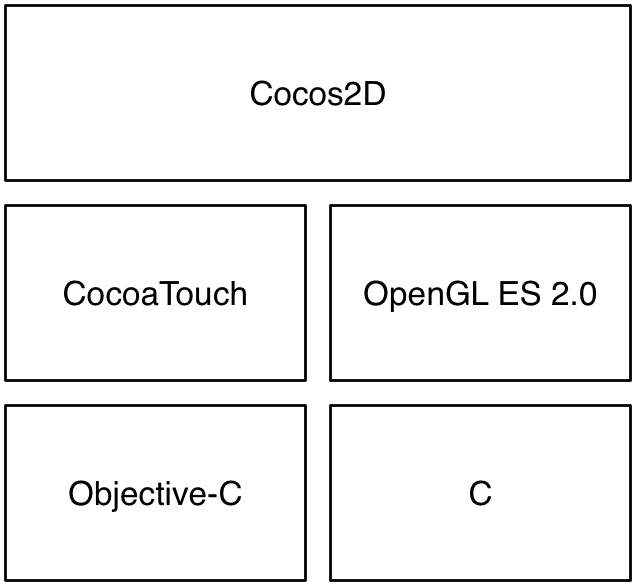
\includegraphics[width=120pt]{images/cocos2d/TechnologyStack.png}     
		\caption{\cocos{} Technology Stack}
\end{figure}

The goal of a game engine like \cocos{} is that the game developer doesn't have
to get in touch with rendering at all. Instead a developer defines which scenes
exist in a game, which nodes are part of these scenes and which size, position
and appearance these nodes have and \cocos{} will use OpenGL to render these
scenes for him.

In order to provide this functionality \cocos{} consists of variety of classes -
some important ones will be discussed in this chapter. All \cocos{} classes use the \textit{CC} prefix (\ccscene{}, \ccnode{}, etc.).

When working with a 2D game engine for the first time you will be introduced to
a whole set of new terminology. We have already talked about nodes and scenes
but we haven't discussed what these terms mean. We will now start discussing the
most important terms and get to know how the concepts behind them are
implemented in \cocos{}.

\subsubsection{How are games rendered in \cocos{}?}
The most important aspect of \cocos{} is that it
\ldots \textbf{addmore}

\subsection{Scenes}
Scenes are the basic building blocks of all \cocos{} games, they are the
highest level on which game content can be structured. Each scene in \cocos{} is
a full-screen canvas. For every full-screen section of your game you will use
\textit{one} scene.
\textbf{Add screenshots here}
Here's an example from the MakeGamesWithUs game \textit{Deep Sea Fury}:
% add image
You can see that the game consists of the start scene, the gameplay scene and
the game over scene.

Scenes are represented by the \ccscene{} class. Another
important \cocos{} class for scene handling is \ccdirector{}. The \ccdirector{}
class is responsible for deciding which scene is currently active in the game
(\cocos{} only allows one active scene at a time). Whenever a developer wants to
display a scene or transition between two scenes he needs to use the
\ccdirector{} class.

This means creating and displaying a new scene is a two step process:
\begin{enumerate}
\item Create a new instance of \ccscene{}
\item Tell the \ccdirector{} to display this new scene
\end{enumerate}

You will learn a lot more about this down the road, but the important bottom
line is: \textit{Scenes are the highest level of structure in your game and a
class called \ccdirector{} decides which scene is currently displayed}.

\subsection{Nodes}
Everything that is visible in your \cocos{} game (and a couple of invisible
objects) are \textit{nodes}. Nodes are used to structure the content of a scene.
Every node can have other nodes as its children. \cocos{} provides a huge amount
of different node types. Every node type is a subclass of \ccnode{}.

Most nodes are used to represent an object on the screen (an image, a solid
color, an UI element, etc.), a few other nodes are only used to group other
nodes. All nodes have a size, positions and children (and many other properties
which are less important for us right now). Here are some of the popular
node types of \cocos{}:

\begin{description}
  \item[CCSprite] represents an image or an animated image. Used for characters,
  enemies, etc.
  \item[CCColorNode] a node being displayed in one plain color.
  \item[CCLabelTTF] a node that can represent text in any TTF font.
  \item[CCButton] a interactive node that can receive touches.
\end{description}

Nodes and their children form a scene graph. The concept of a scene graph isn't
unique to \cocos{} it is a common concept of 2D and 3D graphics. A scene graph
is a hierarchy of many different nodes. 

\subsection{Scene Graphs}
Let's take a look at simple example of a scene graph:

\begin{figure}[H]
		\centering
		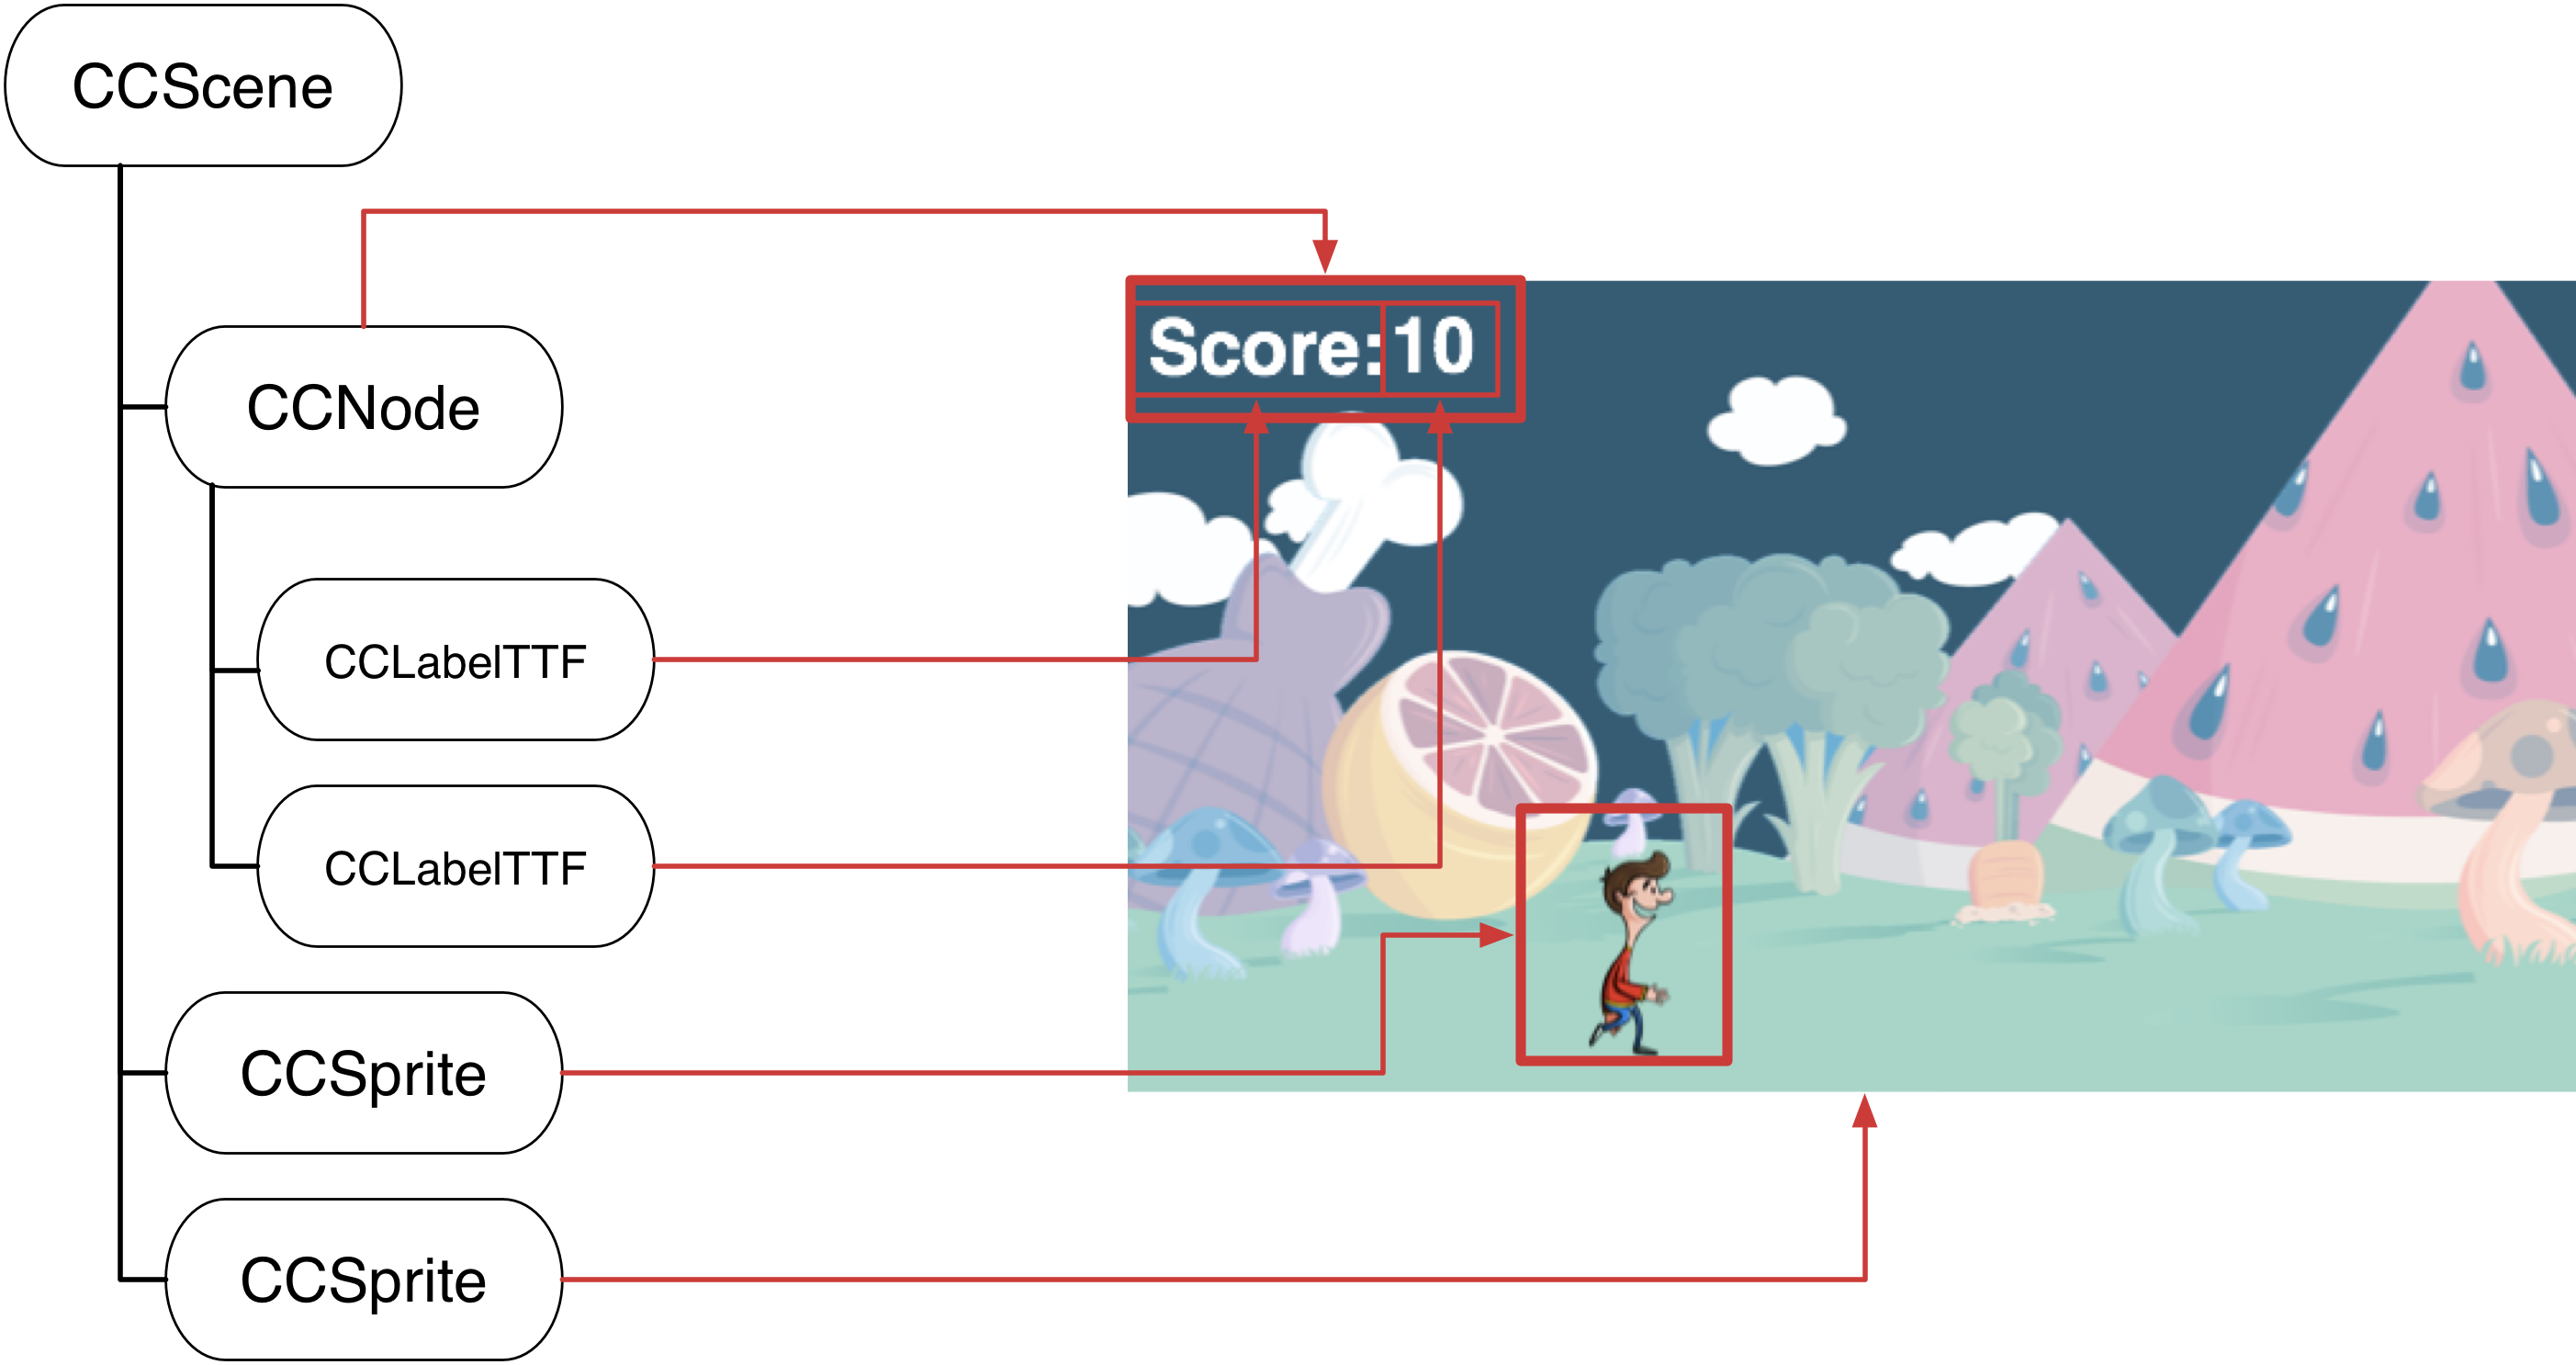
\includegraphics[width=0.9\linewidth]{images/cocos2d/SceneGraph.png}     
		\caption{\cocos{} Scene Graph}
\end{figure}

On the left side of the image you can see the node hierarchy. On the first level
you have the \ccscene{}. As the first child we have a \ccnode{} with two
children of type \cclabel{}. This \ccnode{} is the first example of a grouping
node, it groups the score caption label and the label displaying the actual
score. Instances of \ccnode{} don't have any appearance they are solely used to
group other nodes. Throughout this book you will learn that it often makes sense
to group nodes under certain parent nodes. The main reason is that all children are placed
\textit{relative} to their parents. So if we would want to move the scoreboard
of the example above to the top right corner we would only have to move the
parent node instead of both child nodes. As you can imagine this becomes
even more relevant in games that have ten or more entries in their scoreboard.

\begin{bestpractice}[frametitle={Structuring Nodes}] 
Always group nodes that logically belong together under one parent node. That
will save you a lot of time when you change the layout of your scene.
\end{bestpractice}

The other two objects in the scene graph are simpler. One represents the
background image the other one the main character.

For some games, scene graphs can get very complex and include hundreds of
different nodes. The key takeaways for now are:

\begin{enumerate}
  \item Every node in \cocos{} can have children
  \item A hierarchy of nodes is called a scene graph
  \item Children of nodes are placed relative to their parents - often it is
  useful to group nodes that are moved together under one parent
\end{enumerate}

As you can see nodes are the most important building block of \cocos{} games -
they are used to build everything that is visible in your game. Because it
is so important to understand how nodes work in \cocos{} we will take a look at
the most important properties and methods that \ccnode{} provides.

\subsection{An Introduction to CCNode}\label{Introduction_CCNode}
Every visible object in your game will be a subclass of \ccnode{}. Because
you use nodes to build and arrange your scenes it is important to understand
how nodes are positioned and how positions of nodes can be accessed. Let's
discuss the most relevant properties and methods to access and change
size and position of a \ccnode{}:

\begin{description}
\item[contentSizeInPoints] the size of this node in points
\item[positionInPoints] the position of this node in points, expressed relative
to the parent of this node
\item[anchor point] the anchor point is the center point for rotations and the reference point for positioning this node
\item[boundingBox] the bounding box is a rectangle that encloses a node. You can
only read it but not set it
\end{description}

The \textit{contentSizeInPoints} and \textit{positionInPoints} properties
express the size and the position of a \ccnode{} and should be fairly easy to
understand. The \textit{bounding box} and the \textit{anchor point} however, are
concepts related to game development and these may be new to you. The bounding
box is a rectangle that encloses the entire node, you will see an example of a
bounding box in the next diagram. The anchor point is relevant for positioning
and rotating nodes.

Let's take a look at how anchor points influence positioning first. We know that
the position of a node is expressed relative to its parent. More specifically every node position in
\cocos{} is expressed from the \textit{position reference corner} of the parent
to the anchor point of the \ccnode{}. Here's a visual example in which a bear
node is placed relative to a background node:

\begin{figure}[H]
		\centering
		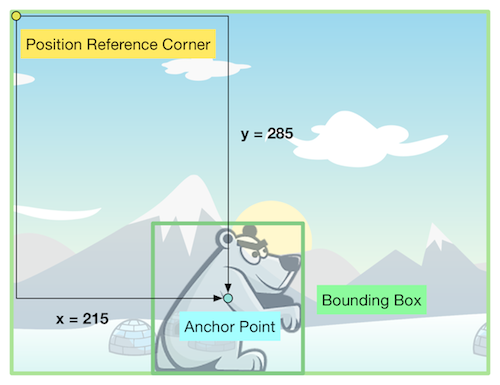
\includegraphics[width=0.5\linewidth]{images/cocos2d/ccnode/NodePositioning.png}     
		\caption{\ccnode{} positioning example}
\end{figure}

As you can see, the \textit{anchor point} and the \textit{position reference
corner} influence the position of a node. The anchor point can have any value
between (0, 0), representing the bottom left corner of a node and (1,1),
representing the top right corner of a node. In the example above, the bear has
a anchor point of (0.5, 0.5) which is at the center of the bear. By choosing an
anchor point of (0.5, 0.5), the \textit{center} of the bear will be positioned
at (215, 285). If we would choose an anchor point of (0,0) the \textit{bottom
left} corner of the bear would be positioned at (215, 285).

The \textit{position reference
corner} lets us define from which of the four corners of the parent node we are
expressing the position of a node. In the example above the top left corner is
the \textit{position reference corner}. We will discuss how to use position reference corners when we start 
creating games that shall work on multiple screen sizes.

The anchor point is not only important for the positioning of a node. It has a
second important function - it represents the center of rotation for a
\ccnode{}. Every \ccnode{} rotates around its own anchor point. Here's an
example of rotating the bear node with two different anchor points:

\begin{figure}[H]
		\centering
		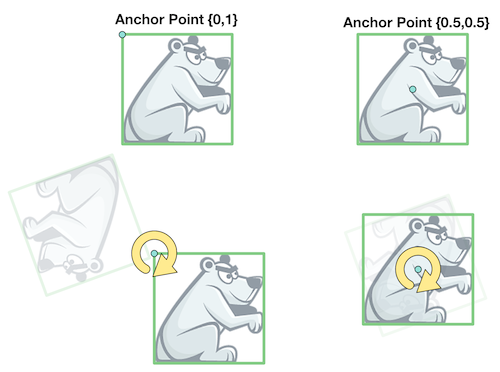
\includegraphics[width=0.6\linewidth]{images/cocos2d/ccnode/Rotation.png}     
		\caption{\ccnode{} positioning example}
\end{figure}

There is a lot more to learn about \ccnode{}, but for now our only goal is to
get a basic understanding of how \cocos{} games are structured and what the most
important parts of \cocos{} are.

You now know that \cocos{} game are structured into scenes. You know that
everything visible in your game is a \ccnode{} and that every \ccnode{} can have
multiple children. You also got a basic understanding of how nodes are
positioned in \cocos{}.

Now that you have that basic understanding, we will take a look at a second tool which we will be using throughout this book: \SB{}.

\section{Introduction to \SB{}}
You have learned the fundamentals of the game engine we will use. Now we will
take a look at a tool called \SB{} which we will use to create the majority of
our game content. The main purpose of \SB{} is to provide a visual editor for
the creation of scenes, animations and more. For most games you will create some
basic mechanics in code (enemy movement, score mechanism, etc.) but you will create
 most of your game content in \SB{} since it is a lot easier to create
levels, menus and other scenes in an editor that provides you with a live
preview instead of putting these scenes together in code.

If you have never used \SB{} before, it is very important to understand that
everything that can be implemented in \SB{} can also be implemented in code.
\SB{} is not part of the game engine, it just allows you to configure \cocos{}
scenes and nodes in an editor instead of configuring them in code.

\subsection{Creating a first project}
To dive into the features of \SB{} we will create our first project! 
Create a new project by opening SpriteBuilder and selecting \textit{File > New >
Project...}:
\begin{figure}[H]
		\centering
		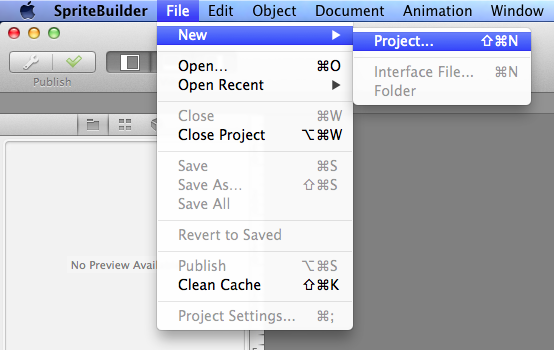
\includegraphics[width=0.9\linewidth]{images/cocos2d/setup/spritebuilder_new_project.png}     
\end{figure}

\SB{} will ask for a name and a location for the new project. Name it
\textit{HelloSB}. After you create the project the folder structure should look similar to this:
\begin{figure}[H]
		\centering
		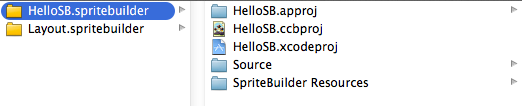
\includegraphics[width=250pt]{images/cocos2d/setup/project_structure.png}     
		\caption{\SB{} project folder structure}
\end{figure}

Every \SB{} project is contained in a \textit{.spritebuilder} folder. Within
this folder all the files of the \SB{} project are stored - along with an \xcode{}
project. 

\begin{lamp}[frametitle={\SB{} and Xcode}] 
\SB{} will create an \xcode{} project for every new project you create! The
\xcode{} project will automatically contain the newest version of \cocos{} -
very handy.
\end{lamp}

Later on you will learn more about how the \SB{} project and the \xcode{}
project work together. The general rule is that all code will be part of the
\xcode{} project and most content creation will happen in the \SB{} project.

\subsection{The Editor}
When you have created your first \SB{} project you will see that the \SB{} UI
gets enabled. Let's take a look at the different parts of the editor to get a
better understanding of \SB{}.

The \SB{} interface is divided into 4 main sections:
\begin{figure}[H]
		\centering
		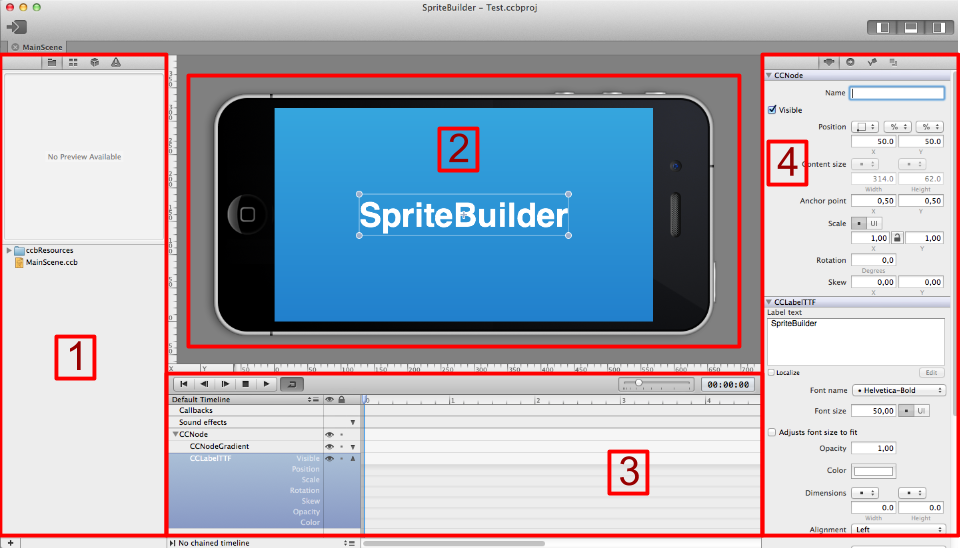
\includegraphics[width=0.9\linewidth]{images/spritebuilder/spritebuilder_ui.png}     
\end{figure} 
\begin{enumerate}
  \item \textit{Resource/Component Browser:} Here you can see the different
  resources and scenes you have created or added to your project. You can also select different types of Nodes and drag them into your scene.
  \item \textit{Stage:} The stage will preview your current scene. Here you can
  arrange all of the nodes that belong to a scene. 
  \item \textit{Timeline:} The timeline is used to create animations within
  SpriteBuilder.
  \item \textit{Inspector:} Once you select a node in your scene, this detail
  view will display a lot of editable information about that node. You can modify positions, content (the text of a label, for example) and physics properties.
\end{enumerate}
Let's take a closer look at some of the most important views.

\subsubsection{File View}
The first tab in the resource/component browser represents the \textit{File
View}.
It lists all the \textit{.ccb} files and resources that are part of the \SB{}
project:
\begin{figure}[H]
		\centering
		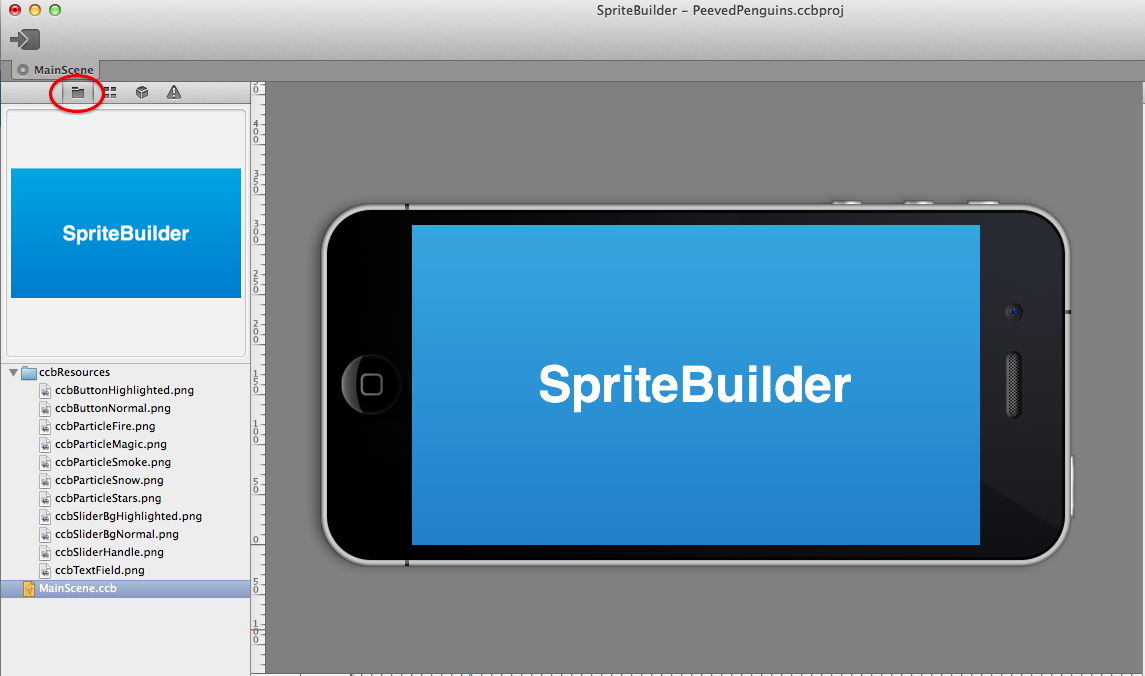
\includegraphics[width=0.8\linewidth]{images/spritebuilder/spritebuilder_fileview.png}     
\end{figure} 
In this view you can add new resources and restructure your project's folder
hierarchy.
\subsubsection{Node Library}
The third tab in the left view is the {Node Library}:
\begin{figure}[H]
		\centering
		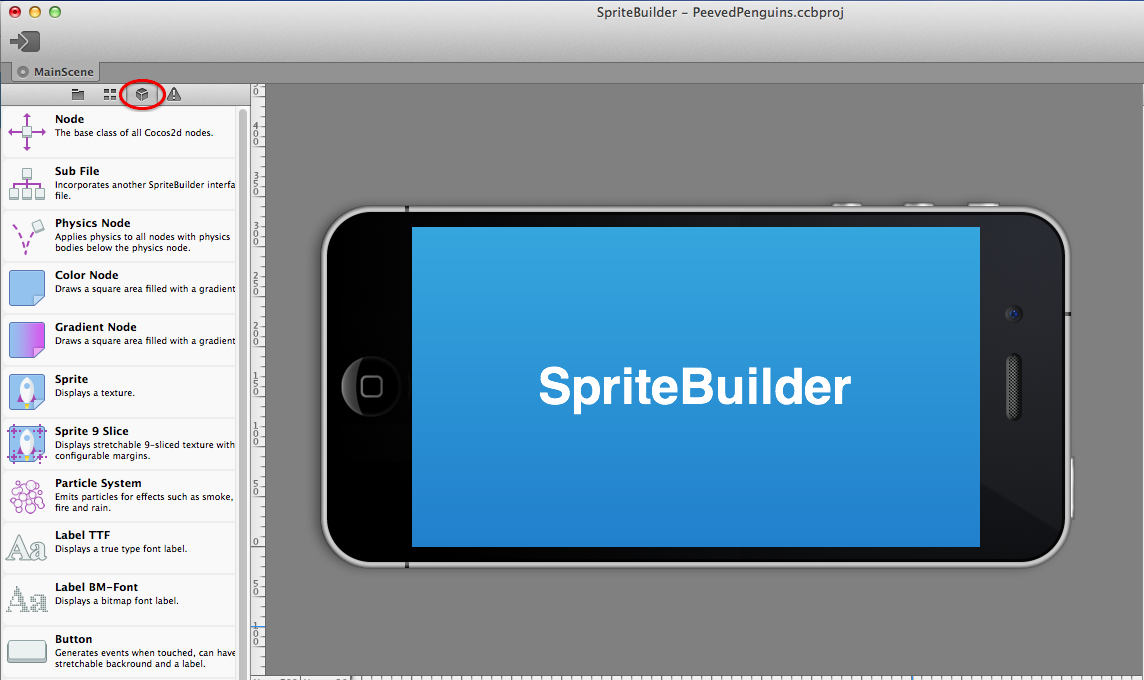
\includegraphics[width=0.8\linewidth]{images/spritebuilder/spritebuilder_nodeview.png}     
\end{figure} 
This panel shows you all available node types you can use to construct your
Gameplay scenes and menus. You will drag these nodes from this view to the stage
in the center to add them to your scenes.

\subsubsection{Inspector}
The first tab of the Detail View (the right panel) is
the Inspector. Once you have selected an object on your stage you can use this panel to modify many of its properties, like position and color:
\begin{figure}[H]
		\centering
		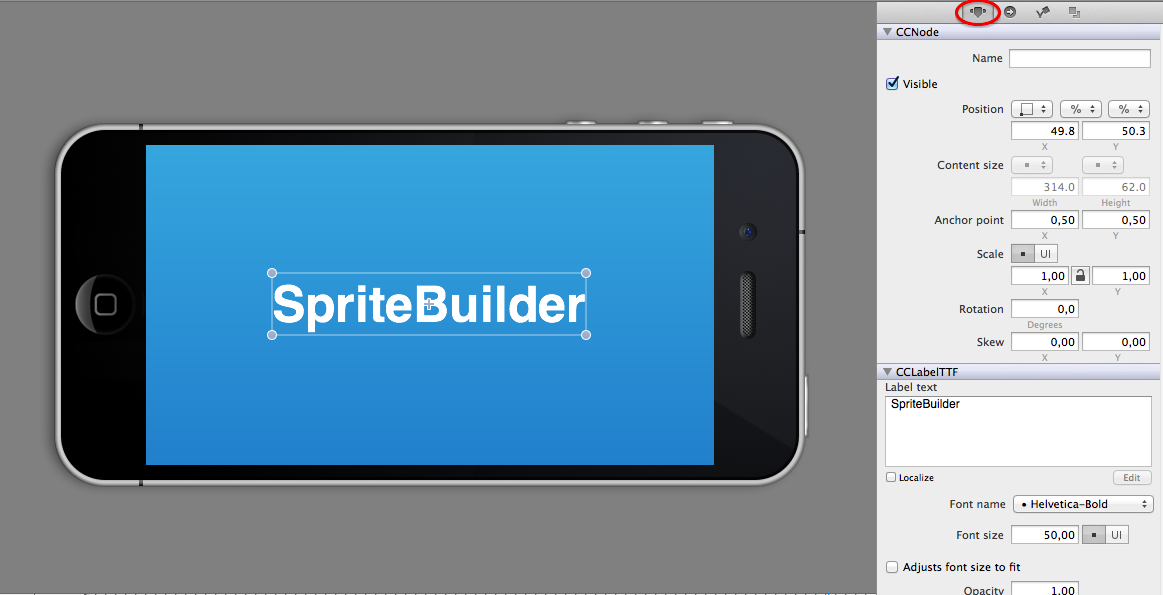
\includegraphics[width=0.8\linewidth]{images/spritebuilder/spritebuilder_inspector.png}     
\end{figure} 

\subsubsection{Code Connections}\index{Code Connections} 
The second tab on the right panel let's you manage code connections for your
selected node. As mentioned previously the entire code for your games will be
written as part of the \xcode{} project. This view allows you to create
connections between the \xcode{} project and the \SB{} project. For example you can set a custom Objective-C class for a node or you can select
a method in your code that shall be called once a button in your scene is tapped. 

\begin{figure}[H]
		\centering
		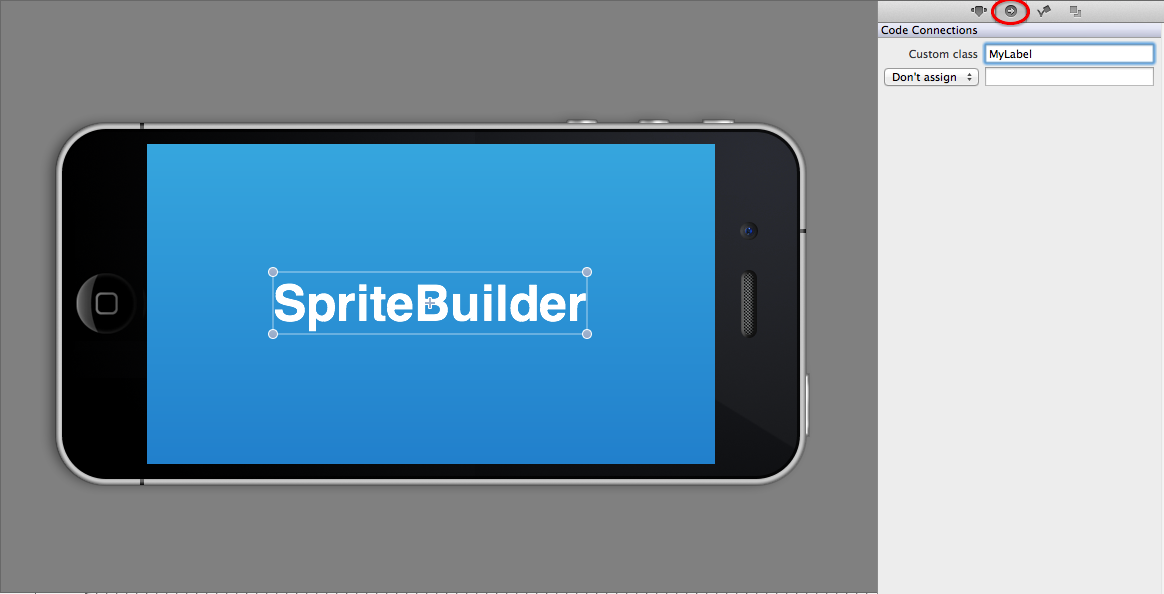
\includegraphics[width=0.8\linewidth]{images/spritebuilder/spritebuilder_codeconnections.png}     
\end{figure} 
Code connections will be discussed in detail later on.

\subsection{\ccbfile{}s}
\ccbfile{}s are the basic building blocks of your \SB{} project. Every scene in
your game that is created with \SB{} is represented by one \ccbfile{}. However
\ccbfile{}s are not only used to create entire scenes - they are used to create
any kind of scene graph. \SB{} provides different kinds of document types
depending on which type of scene graph you want to create. You get an overview of the
available \ccbfile{} types when you create a new one, by selecting
\textit{New > File... } from the \textit{File} menu in \SB{}:
\index{Document Types}\label{DocumentTypes}
\begin{figure}[H]
		\centering
		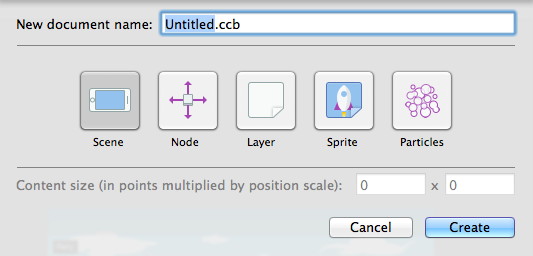
\includegraphics[width=240pt]{images/spritebuilder/new-ccb.png}     
\end{figure} 
These are the different document types briefly explained:
\begin{description}
\item[Scenes] will fill the full screen size of the device.
\item[Nodes] used primarily for grouping functionality, don't have a size.
\item[Layers] are nodes with a content size. This is useful, for instance, when
creating levels or contents for scroll views.
\item[Sprites] used to create (animated) characters, enemies, etc.
\item[Particles] is used to design particle effects.
\end{description}
You will get a good understanding when to use which type of \ccbfile{} once we
get started with our example projects. The key takeaway is that \ccbfile{}s are
used by \SB{} to store an entire scene graph including size, positions and many
other properties of all the nodes that you have added.

\subsection{How \SB{} and \xcode{} work together}
\label{Publish}
I have mentioned how \SB{} and \xcode{} integrate a couple of times briefly. In
order to be a well versed and efficient \SB{} game developer it is very
important to understand the details of this cooperation.

When creating a \SB{} project, \SB{} will create and maintain a corresponding
\xcode{} project. In \SB{} will you create multiple \ccbfile{}s that describe
the content of the scenes in your game. You will also add the resources that
you want to use in your game and set up code connections to interact with the
code in your \xcode{} project. \xcode{} will be the place where you add code to
your project and where you run the actual game.

Since \xcode{} is the tool that actually compiles and runs your game it needs
to know about all the scenes and resources that are part of your \SB{} project.
Therefore \SB{} has a \textbf{publish}\index{Publish} functionality, provided by
a button in the top left corner of the interface:
\begin{figure}[H]
		\centering
		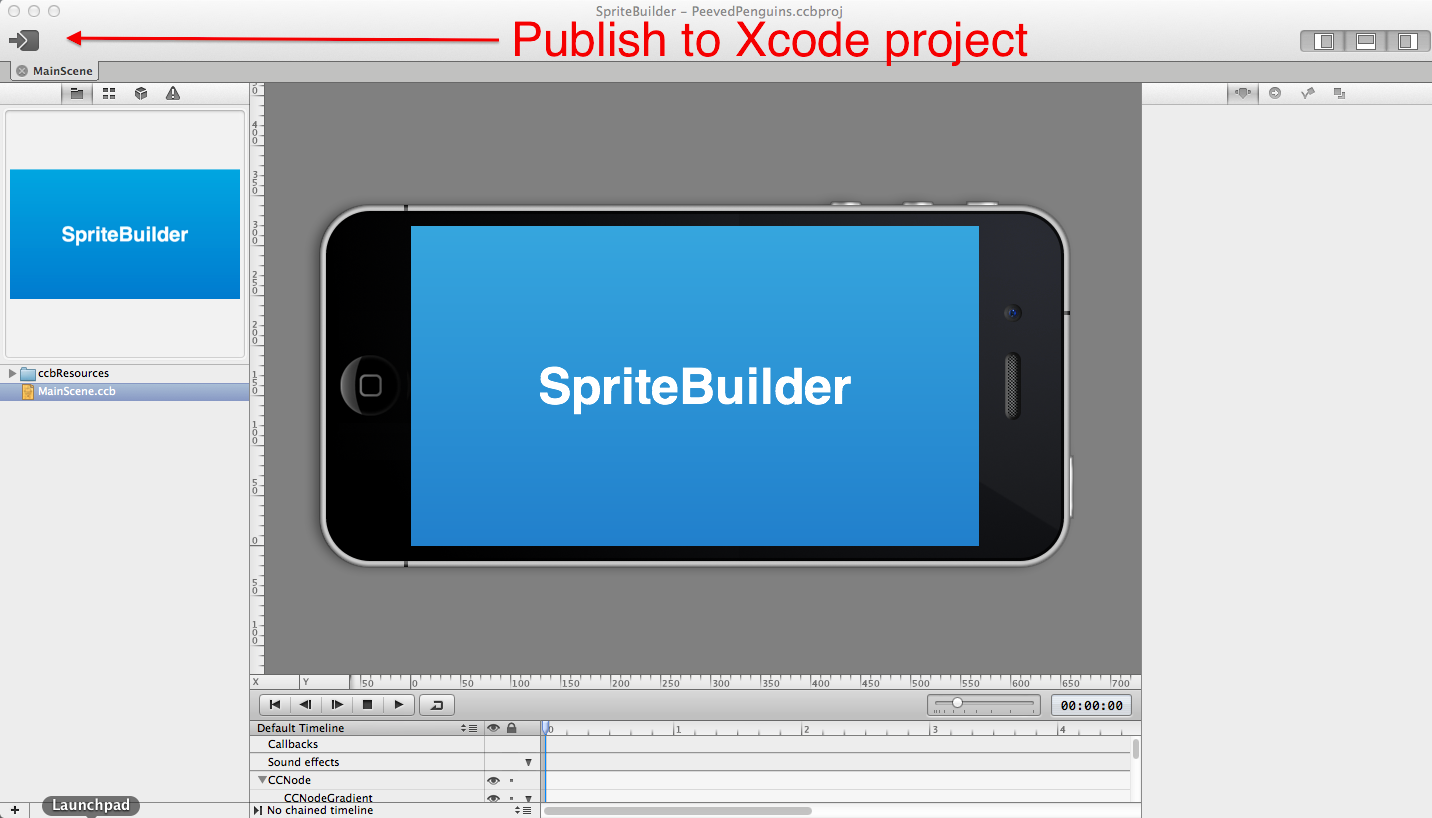
\includegraphics[width=0.9\linewidth]{images/spritebuilder/spritebuilder_publish_button.png}
		\caption{Use the publish button to update your \xcode{} project with the
		latest changes in your \SB{} project.}
		%\label{labelstruct} 
\end{figure}
Using that button, you publish your changes in your
\SB{} project to your \xcode{} project. Whenever you changed your \SB{}
project and want to run it you should hit this button before building the \xcode{}
project.

Here's a diagram that visualizes how \SB{} and \xcode{} work together:
\begin{figure}[H]
		\centering
		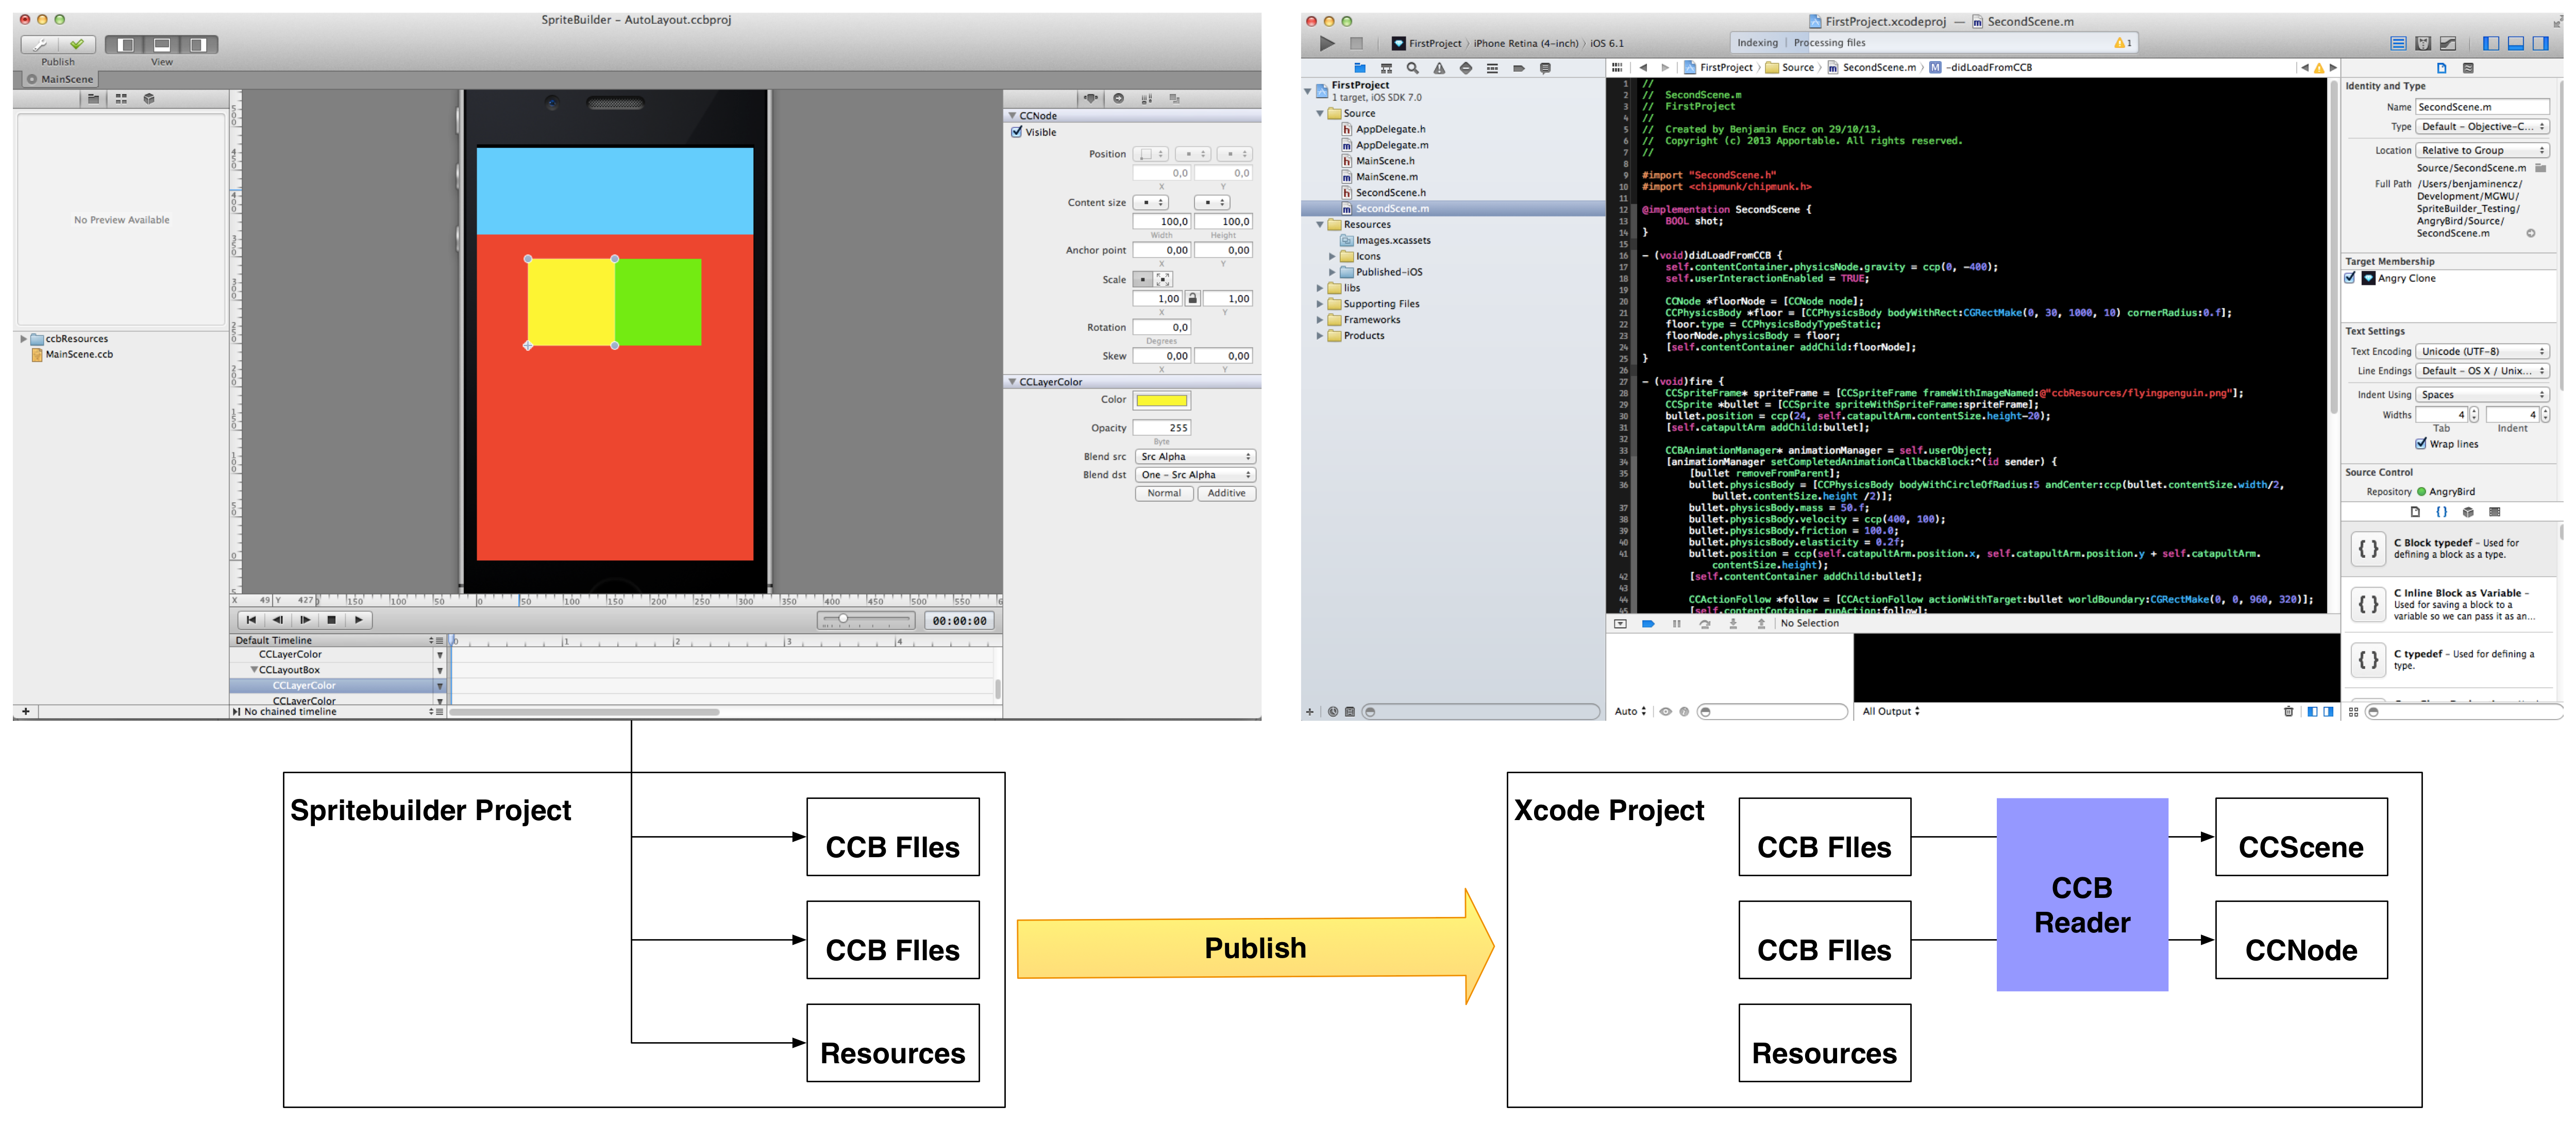
\includegraphics[width=0.9\linewidth]{images/spritebuilder/spritebuilder_publishing.png}
		\caption{\SB{} creates and organizes a \xcode{} project for you. Adding
		all the resources and scenes you have created.}
		%\label{labelstruct} 
\end{figure}
\ccbfile{}s created in \SB{} store a scene graph; the hierarchy and positions of
your nodes. When publishing a \SB{} project the \ccbfile{}s and all other
project resources are copied to your \xcode{} project.
\label{CCBReader}
When running the project in \xcode{} a class called CCBReader will parse your
\ccbfile{}s and create the according \ccnode{} subclasses to reconstruct the scene
graph you have designed in \spriteb{}.

If you would use \cocos{} without \SB{} you would manually create instances of
\ccnode{}, \ccsprite{}, etc. in code and add children to these nodes -
essentially building the entire scene graph in code.

When using \SB{} the CCBReader class will build this scene graph for you, based
on the information stored in the \ccbfile{}s that you created in \SB{}.

Another important part of information contained in \ccbfile{}s that we have not
discussed in detail yet are \textit{Code Connections}.

\subsection{Code Connections}
\label{CodeConnections}
Code connections are used to create links between your scenes in \SB{} and your
code in \xcode{}. There are three basic types of code connections:
\begin{description}
\item[Custom Classes] are an important information for the CCBReader. As
mentioned previously the CCBReader builds the scene graph by creating different
nodes based on the information in your \ccbfile{}. By default it will create an
instance of \ccsprite{} for every sprite you added in \SB{} an instance of \ccnode{} for every node you added, etc. Often
however you will want to add custom behaviour to a node (for example a movement
pattern for an enemy). Then you will have to use the \textit{Custom Class}
property to tell the CCBReader which class it should instantiate instead of the
default one. Whichever class you enter here needs to be a subclass of the
default class (e.g. a subclass of \ccsprite{}). You will learn how to use this
feature in the final project of this chapter!
\item[Variable Assignments] If you have assigned a \textit{Custom Class} you can
use variables assignments to retrieve references to different nodes in the
scene. For example a character might want a reference to its right arm node (a
child of the character node) in order to move it. 
\item[Callbacks] are only available to UI elements like buttons and sliders.
They allow you to decide which method should be called on which class once a
button is pressed.
\end{description}
Now you should have an idea about what code connections are used for and which
kinds exist. We will discuss the details of all types when we use them as part
of our example projects.

\section{A first \SB{} project} 
You have already created the \SB{} project called \textit{HelloSB}. Now we will
start adding some content to it. The project built in this chapter will consist
of two scenes one start screen and one game screen. In the game screen the user will be able to spawn randomly
colored squares that rotate, by tapping on the screen.
\begin{figure}[H]
		\centering
		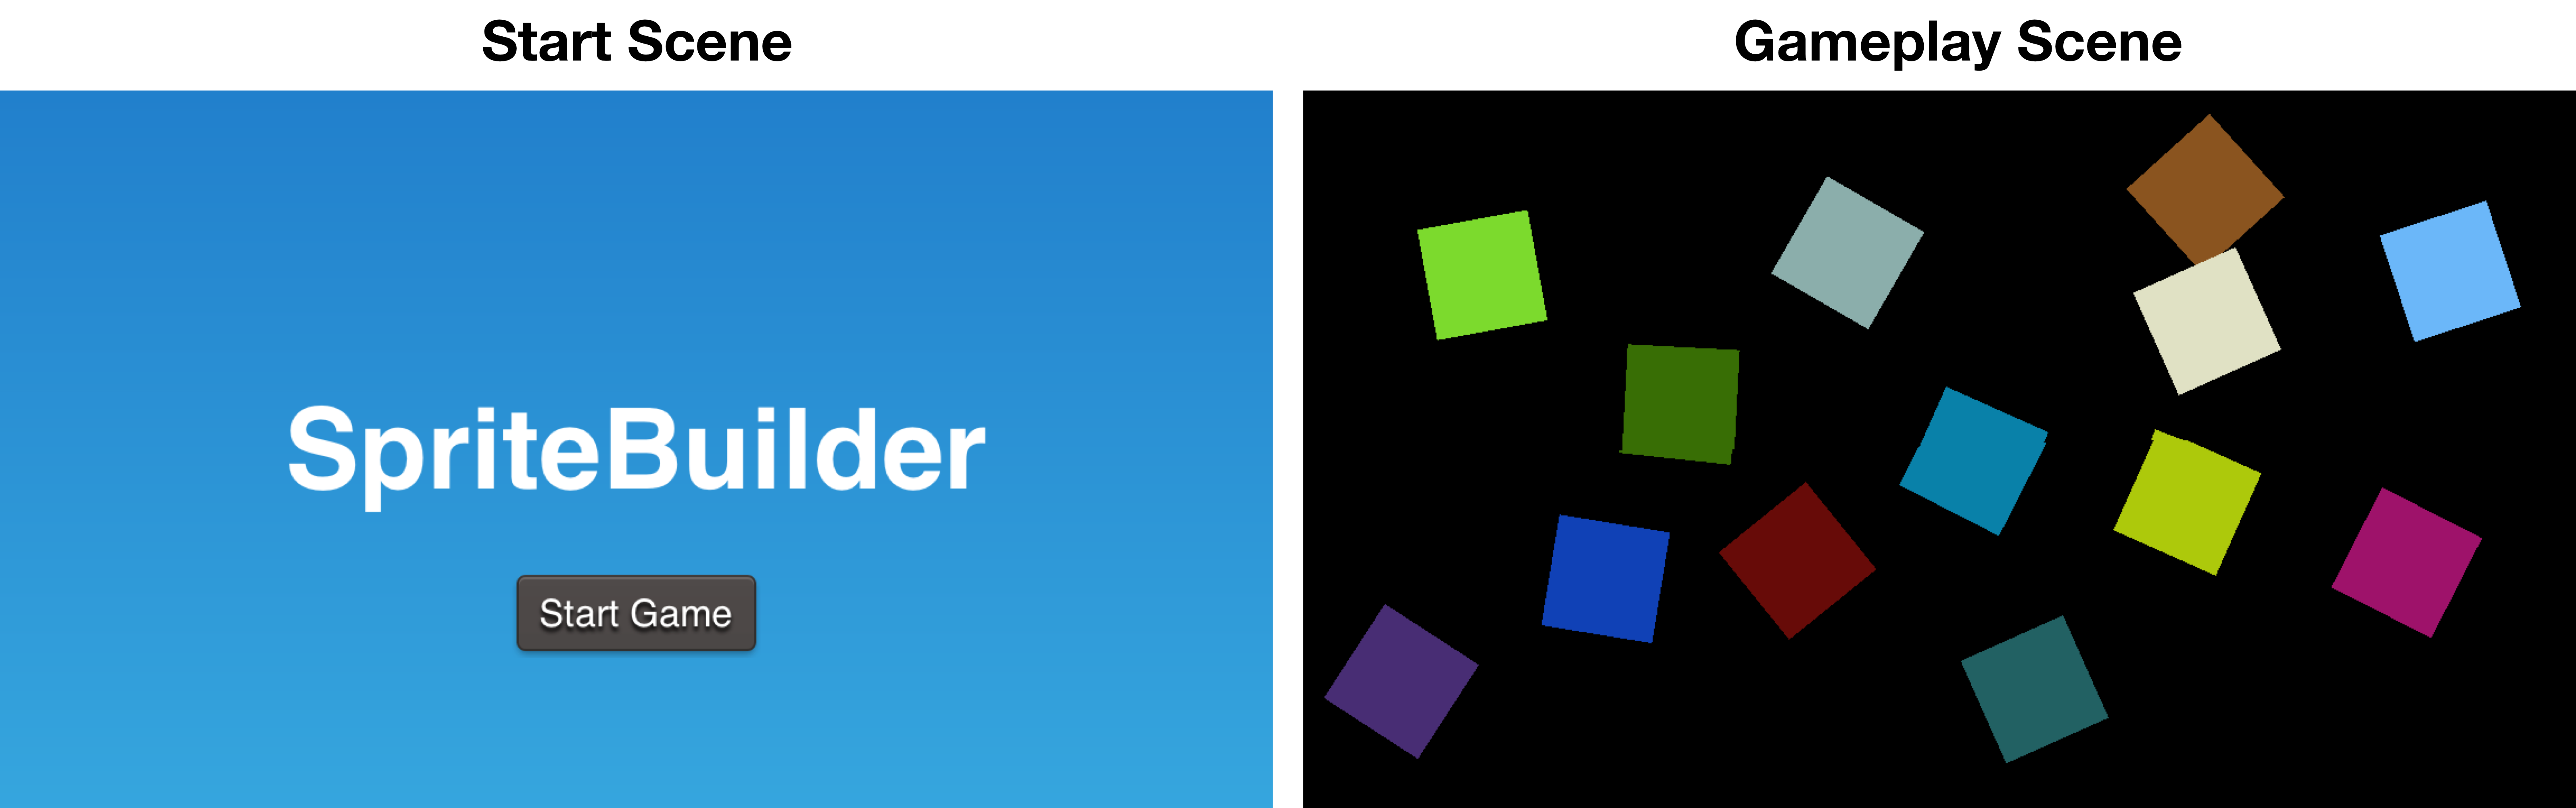
\includegraphics[width=0.9\linewidth]{images/firstproject/first_project.png}
		\caption{The project build throughout this chapter}
		%\label{labelstruct} 
\end{figure}
By creating this project you will learn all of the following:
\begin{itemize}
  \item Creating scenes in \SB{}
  \item Creating code connections (callbacks, variable assignments and custom
  classes)
  \item Switching between different scenes
  \item Manipulate a scene graph from code (add/remove nodes, load CCB Files and
  add them to the scene)
  \item Use the \cocos{} action system to create animations
  \item Use the \cocos{} touch handling system to capture touches
\end{itemize}

\subsection{Setting up the first scene}
%explain code connections in detail here
Now it is time to open the \textit{HelloSB} \SB{} project. We want to add a
\textit{Start Button} to the first scene. When this button is tapped we want to
switch to the second scene. 

\subsubsection{Positioning the first button}
Start by adding a button to the first scene:

\begin{figure}[H]
		\centering
		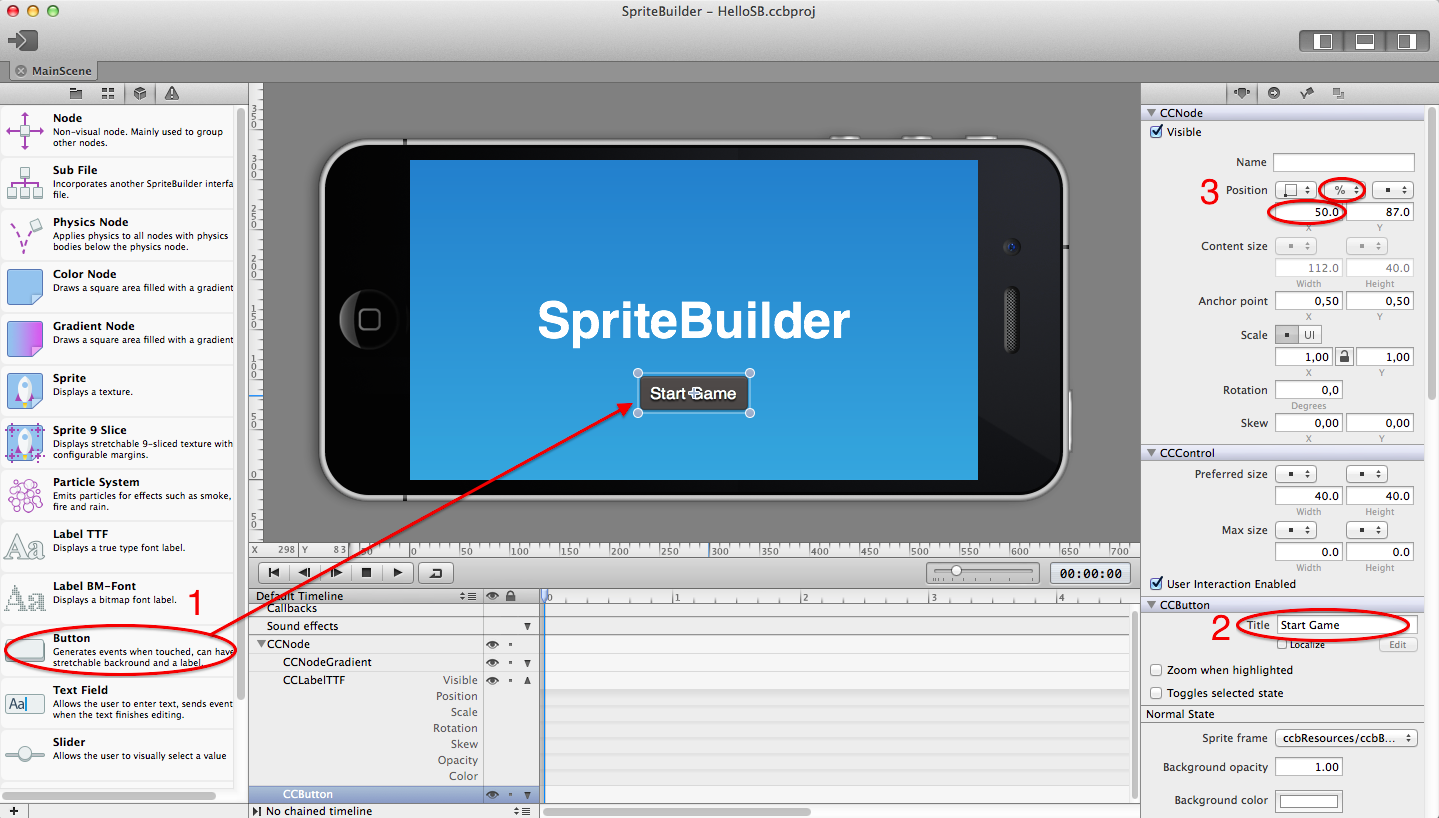
\includegraphics[width=0.9\linewidth]{images/firstproject/add_button.png}
		\caption{The project build throughout this chapter}
		%\label{labelstruct} 
\end{figure}

One simple button, but since this is your first action in \SB{} there's
\textit{lots} to explain about it. Let's look at the three steps highlighted in
the image above, one by one.

\begin{description}
\item[(1)] Open \textit{MainScene.ccb} by double clicking it in the left
resource pane. Then open the third tab in the left pane, the \textit{Node
Library}. Remember, this section shows you all the different node types
supported by \SB{}. Select the \textit{Button} and drag it over to the stage,
dropping it below the existing label. Dropping it on the stage will add this
node to your scene. Another way of adding a node to a scene is dropping it to
the timeline at the bottom of the screen - we will look at this later.
\item[(2)] Make sure the button is selected, because we want to change some
properties of it. Whenever you have selected a node the right pane will display
all the properties you can edit. Navigate to the \textit{Title} textfield in the
property pane and change the title of the button to \textit{Start Game}.
\item[(3)] So far - so simple. Step number three will expose you to a very
interesting feature of \SB{}: the positioning system. It will allow you to not
only use absolute positions but also positions that are relative to the size of
the parent node. We want to center the button horizontally so we choose the
position type for the X component to be \textit{in percent of parent
container} by selecting that option from the dropdown menu. Now we assign
\textit{50} as value, because that expresses the horizontal center of the parent
container. Whichever screen this button will be displayed on, it will always be
vertically centered (yes, even on an iPad)!
\end{description}

\begin{details}[frametitle={Positioning System in \cocos{} and \SB{}}]
\index{Positioning System} \label{PositioningSystem}
The positioning system in \cocos{} is designed from the ground up to make it
easy to design scenes and user interfaces for different screen sizes and
resolutions. The comfortable days where the 3.5-inch iPhone was the only 
available iOS device and defining layouts with absolute positions was acceptable
are finally over. Today app and game developers face a variety of different
devices and customers justifiably expect your software to work great on all of
them. \cocos{} offers the following properties on \ccnode{}s to allow developers
to design their interfaces with great flexibility:

\begin{itemize}
  \item Anchor Point
  \item Reference Corner
  \item Position Type
  \item Size Type
\end{itemize}

Check the extra chapter on dynamic layouts in \SB{}. %TODO: Add reference, etc.

\end{details}

Now the button is placed correctly. Next, we want to assign an action to it.
When the button is tapped we want to transition to our second scene.

\subsubsection{Setting up a code connection}

Earlier you learned that \SB{} has three types of code connections 
(\ref{CodeConnections}). Now we will use one of them in our project -
\textit{Callbacks}\index{Code Connections!Callbacks}. Callbacks are only
available to nodes that allow for some sort of user interaction (this means they need to be subclasses of
\inlinecode{CCControl}). Buttons, next to Sliders and Text Fields are one of
these types of nodes. Select the button we have added to the scene earlier and
select the third tab of the right pane:

\begin{figure}[H]
		\centering
		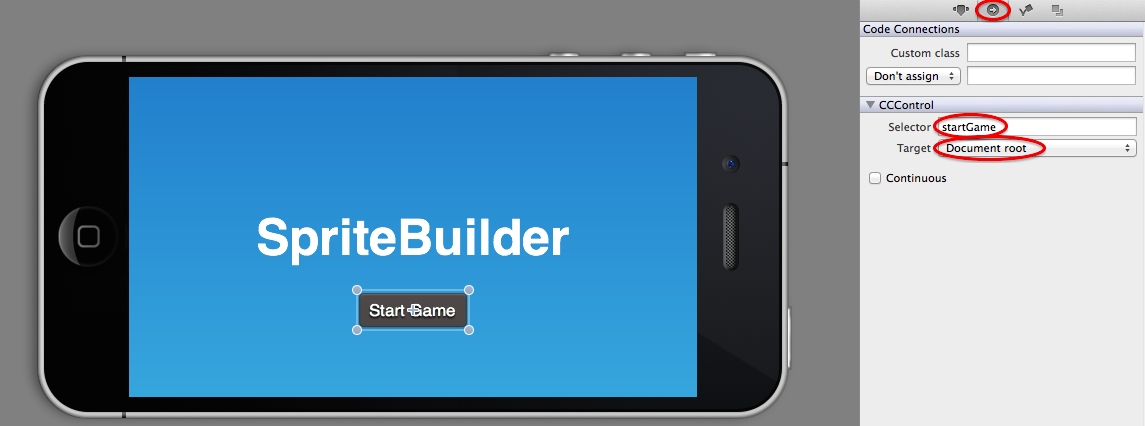
\includegraphics[width=0.9\linewidth]{images/firstproject/button_callback.png}
		\caption{Nodes that allow user interaction can use callback methods to
		connect to the code base}
		%\label{labelstruct} 
\end{figure}

Inside the CCControll section you can see two options called \textit{selector}
and \textit{target}. Here you can choose which method (selector) shall be
called on which object (target) when this button is tapped by a user. As
selector enter \inlinecode{startGame}. As target choose \textit{Document Root}.

\begin{details}[frametitle={Targets and Selectors}] \label{target_selector}
The concept of targets and selectors is part of design pattern widely used
throughout the Cocoa framework (Target/Action pattern). A \textit{selector} is
a method name and a \textit{target} is the object that shall receive this method.
Further reading:
\url{https://developer.apple.com/library/ios/documentation/general/conceptual/Devpedia-CocoaApp/TargetAction.html}
\end{details}

As you can see you cannot choose an arbitrary object to be the target of this
callback, you can only choose between two different ones:
\begin{description}\label{DocumentRoot_Owner}
\item[Document Root] The document root\index{Document Root} is the highest node
within the current \ccbfile{}. The hierarchy of the \ccbfile{} is shown in the
\SB{} timeline: \begin{figure}[H]
		\centering
		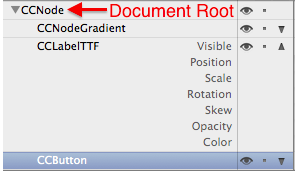
\includegraphics[width=150pt]{images/firstproject/documentroot_node.png}
		%\label{labelstruct} 
\end{figure}
If you select the document root as target, the \inlinecode{startGame} method
will be called on the top level \ccnode{}. 
\item[Owner] if you want the callback to call an object that is not part of your
\ccbfile{} you can use the \textit{owner} option. Later in this book you will
learn how to set up an owner object for a \ccbfile{}.
\end{description}

For our button we have decided that the \inlinecode{startGame} method should be
called on the document root when the button is tapped. Next, we will have to
implement this \inlinecode{startGame} method within our document root. But to
which \textit{class} could we add this method? In order to find that out we need to understand the
concept of \textit{Custom Classes} \index{Code Connections!Custom Classes}.
Think about it - by default our document root is an instance of a plain
\ccnode{} class.
Now we want to call a method called \inlinecode{startGame} on this object. Our
problem: the \ccnode{} class does not have a \inlinecode{startGame} method! This
is where custom classes come to rescue us, they allow us to tell \SB{} that our
document root node should \textbf{not} be a plain \ccnode{} but should be an
instance of a class that we have created and that knows about our
\inlinecode{startGame} method. To define a custom class for the document root
you need to select the document root (the top-level \ccnode{}) from the timeline
and open the third tab in the right pane:

\begin{figure}[H]
		\centering
		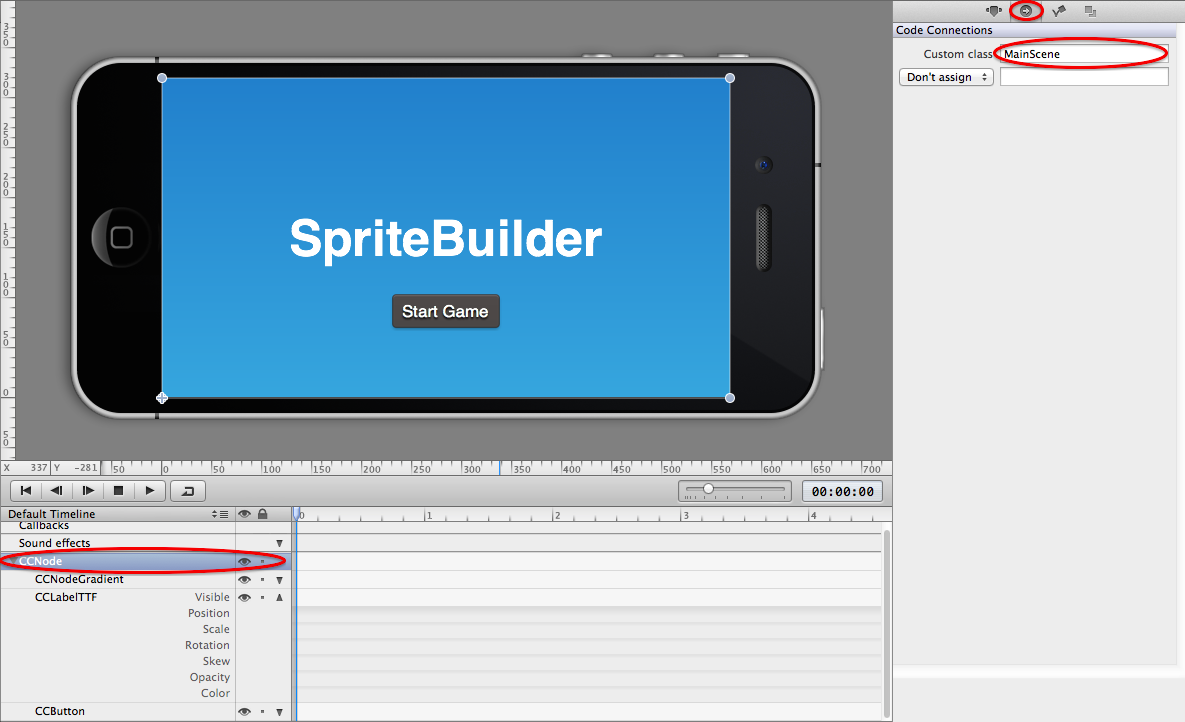
\includegraphics[width=0.9\linewidth]{images/firstproject/custom_class.png}
		%\label{labelstruct} 
\end{figure}

In the \textit{Custom class} textfield a developer can enter a class name. The
class entered here needs to be part of the \xcode{} project related to this
\SB{} project. As you can see every new \SB{} project already comes with a
custom class set up for the root node of \textit{MainScene.ccb}. When the
CCBReader loads this \ccbfile{} it will create an instance of \inlinecode{MainScene} instead of an instance of
\inlinecode{CCNode}.
Now our document root object is a \inlinecode{MainScene} object! That also means
that we have saved the puzzle of where to add the code for the
\inlinecode{startGame} method - it needs to be part of the
\inlinecode{MainScene} class.

\begin{details}[frametitle={Requirements for Custom Classes}] \index{Code
Connections!Custom Classes}
Every custom class has to be a subclass of the default class for a given node.
For example, the default class for the \textit{Sprite} node in \SB{} is
\ccsprite{}. If a developer wants to set a custom class for a Sprite node, that
class has to be a subclass of \ccsprite{}. \textbf{Why?} \SB{} expects custom
classes to only \textbf{add} behaviour to a default class. All the functionality
of the default class should remain available. If your custom class for a Sprite
node doesn't allow \SB{} to set an image, because it is a subclass of \ccnode{}
the CCBReader and finally also you will run into big problems!
\end{details}

\subsubsection{Adding Code to a \SB{} project}
When creating games with \SB{} we are always working with two tools. \SB{} to
create interfaces and scenes (our game content) and \xcode{} to add code (game
mechanics, etc.). Now we will add our first few lines of code to the
\inlinecode{MainScene} class. Now it's time to publish the changes in our \SB{}
project, so that they are available in our \xcode{} project. Use the publish
button in the top left corner of the \SB{} interface (\ref{Publish}). 

Now open the \xcode{} project (it's called \textit{HelloSB.xcodeproj} and is
located inside the \textit{HelloSB.spritebuilder} folder). You will see that
project contains two classes, \inlinecode{AppDelegate} and
\inlinecode{MainScene}. As part of the template for new \SB{} projects the
\inlinecode{MainScene} class has already been created for you. For any
subsequent custom classes you link in your \SB{} project you will need to create
the according class in \xcode{} on your own. 

Now it's finally time to implement the \inlinecode{startGame} method. Open the
\textit{MainScene.m} and file and add the following method:

\begin{lstlisting}
- (void)startGame {
  CCLOG(@"Start Button Pressed!");
}
\end{lstlisting} 

For now we will simply use the \inlinecode{CCLOG} macro to log a text to the
console once the button is pressed, this is an easy way to check if our code
connection is set up correctly.

\begin{lamp}[frametitle={Displaying the console in \xcode{}}] 
To display the console in \xcode{} select \textit{View -> Debug Area ->
Activate Console}.
\end{lamp}

Now, run the \xcode{} project by hitting the play button in the top left corner.
You should check that you have selected \textit{HelloSB} as target and are set
up to run the app on a simulator (indicated by a device description instead of
a device name):
\begin{figure}[H]
		\centering
		
\includegraphics[width=200pt]{images/firstproject/run_app.png}
\end{figure}
Hitting the run button will compile your app and launch it on an iOS simulator.
Once your app is launched, click on the start button and check the console for
the log message. You should see something similar to this:

\begin{figure}[H]
		\centering
		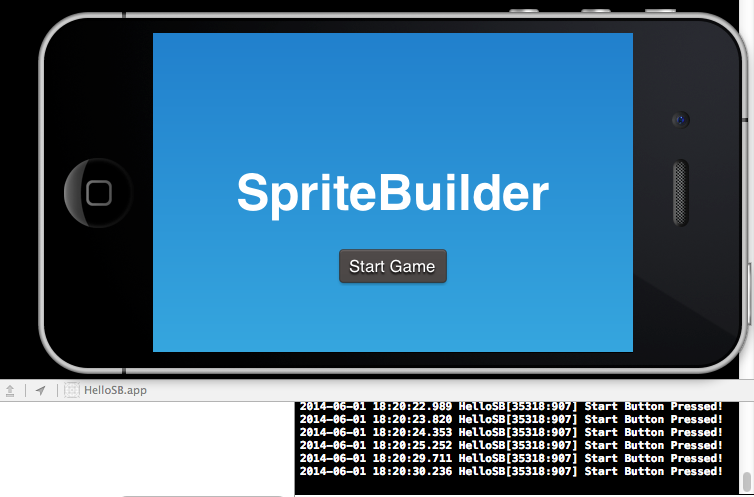
\includegraphics[width=0.9\linewidth]{images/firstproject/button_success_log.png}
		%\label{labelstruct} 
\end{figure}

You have successfully set up your first \SB{} scene and have created a working
code connection! Later on this button shall trigger a transition to the second
scene in the game. Before we can implement that we need to create the second
scene in our \SB{} project!

%TODO: potentially ad recap of how custom class works?

\begin{error}
If you are not getting the expected result, check for all of these common
errors:
\begin{itemize}
  \item Have you published your \SB{} before running in \xcode{}?
  \item Is the custom class of the root node of \textit{MainScene.ccb} set to
  \inlinecode{MainScene}
  \item Does the button in \textit{MainScene.ccb} have the correct target and
  selector?
\end{itemize}
\end{error}

\subsection{Creating the Gameplay Scene}
Now it's time to create your first scene using \SB{} from scratch. The scene we
are going to create is the Gameplay scene. To create a new scene (or any
other \ccbfile{}) select: \textit{File -> New -> File\ldots} from the \SB{} menu.
Then you will see the following dialog appear:

\begin{figure}[H]
		\centering
		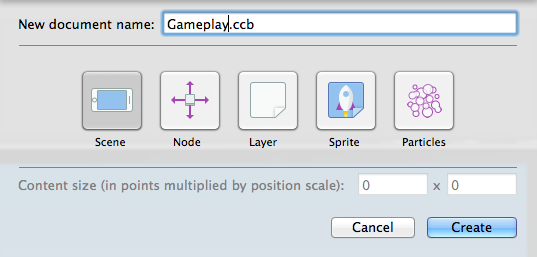
\includegraphics[width=250pt]{images/firstproject/new_scene.png}
		%\label{labelstruct} 
\end{figure}

The dialog will ask you for a name for the \ccbfile{} and a template type. For
now we are going to use the name \textit{Gameplay.ccb} and the type
\textit{Scene}. Once you hit the create button you will see the new, blank
scene appear.

Our Gameplay scene will remain empty. As you have seen in the outline
of the project, we want to dynamically add colored objects to the game, whenever
the user taps into our Gameplay scene - initially however, the scene will be
blank. Now that we have created the Gameplay scene, we can add the transition
from the Main scene to the Gameplay scene.

\subsection{Adding a Scene Transition}
Transitions \index{Scene Transition} are essential for any game. We use them
whenever we want to switch from one scene to another. Transitions cannot be configured in
\SB{}, they always need to be implemented in code. To implement this step,
you need to open your \xcode{} project again.

\cocos{} has one central class that is responsible for displaying the active
scene and generating transitions between different scenes:
\inlinecode{CCDirector}\index{CCDirector}. CCDirector is implemented as a
singleton - thus there's only one CCDirector per \cocos{} game. The instance can be accessed
through the class method \inlinecode{[CCDirector sharedInstance]}.

\begin{lamp}[frametitle={CCDirector is versatile!}] 
CCDirector is responsible for a lot more than only handling active scenes and
scene transitions. It is basically a collection of different global \cocos{}
settings. The scene handling methods however are the most frequently used
CCDirector methods.
\end{lamp}

CCDirector provides a large collection of methods to present scenes with and
without transitions, here are the most important ones:

\begin{lstlisting}
- (void)presentScene:(CCScene *)scene;
- (void)presentScene:(CCScene *)scene withTransition:(CCTransition *)transition;
- (void)pushScene:(CCScene*) scene;
- (void)pushScene:(CCScene *)scene withTransition:(CCTransition *)transition;
- (void)popScene;
- (void)popSceneWithTransition:(CCTransition *)transition;
- (void)popToRootScene;
- (void)popToRootSceneWithTransition:(CCTransition *)transition;
\end{lstlisting}

\cocos{} has two different approaches for displaying a new scene.
\textbf{Replacing} the current scene with a new one, using the
\inlinecode{presentScene:} methods, or \textbf{Pushing} the new scene on top of
the currently active one using the \inlinecode{pushScene:} methods. Whichever
type you choose, you always have the option to provide a transition effect for
presenting a scene, or not to provide a transition effect and display the new
scene instantaneously. If you want to provide an effect you need to create an
instance of \inlinecode{CCTransition}.

Before we look into using transition effects, let's take a look at the
differences between pushing and replacing a scene.

\subsubsection{Replacing scenes vs. pushing scenes}
When you simply want to replace the current scene with a new one you should use
the \inlinecode{presentScene:} method. Here's an example:
\begin{lstlisting}
[[CCDirector sharedDirector] presentScene:myNewScene];
\end{lstlisting}
Very simple! So why would one use the \inlinecode{pushScene:} method?
Let's assume the following scenario where we want to implement a menu with
multiple submenus. Whenever a player hits the back button, he wants to return
to the previous menu:
\begin{figure}[H]
		\centering
		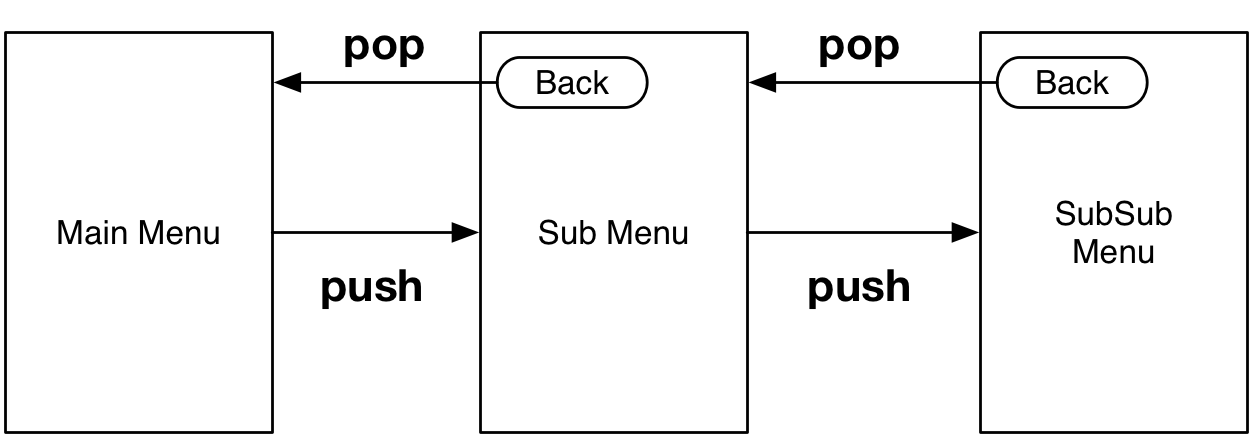
\includegraphics[width=250pt]{images/firstproject/navigation_stack.png}
		%\label{labelstruct} 
\end{figure}
This is a case where it is a lot easier to use \inlinecode{pushScene:} and
\inlinecode{popScene:} instead of simply replacing the currently running scene.
Whenever a player selects a button that opens a sub-menu, we call:
\begin{lstlisting}
[[CCDirector sharedDirector] pushScene:submenu];
\end{lstlisting}
And whenever a player hits the \textit{back} button in one of the sub-menus, we
simply call:
\begin{lstlisting}
[[CCDirector sharedDirector] popScene];
\end{lstlisting}
This works, because CCDirector will remember the scene that we pushed before the
current one and can easily return to it. This concept is called a
\textit{Navigation Stack}.

If you would try to implement the menu hierarchy using
\inlinecode{presentScene:} you would have to explicitly define which scene each
back button will present. The code for the back button of \textit{SubMenu}
would look like this:
\begin{lstlisting}
[[CCDirector sharedDirector] presentScene:mainMenu];
\end{lstlisting}
If you would ever change the menu hierarchy in your game, you would have to
change the code for each back button.

\begin{bestpractice}[frametitle={Scene transitions - the right way}] 
For \textbf{one time transitions} for example from a splash screen to the
gameplay of a game, use \inlinecode{presentScene:}. Whenever a user can navigate
between your scenes, e.g. by using a back button to return to the previous
scene, make use of the navigation stack by using the \inlinecode{pushScene:} and
\inlinecode{popScene:} methods.
\end{bestpractice}

\subsubsection{Adding transition effects}
For every scene replacement method there's one variation that takes an instance
of \inlinecode{CCTransition}. The CCTransition instance provides an animation
for transitions between different scenes. CCTransition provides multiple class
methods to easily create them. Here's an example of how to provide an animated
transition:
\begin{lstlisting}
CCTransition *transition = [CCTransition transitionCrossFadeWithDuration:1.f];
[[CCDirector sharedDirector] presentScene:gameplayScene
withTransition:transition];
\end{lstlisting}

\subsubsection{Implementing a scene transition for our game}
Now that you know the most important details about scene transitions, let's add
the transition from our start scene to our Gameplay scene. Open
\textit{MainScene.m} in \xcode{}. Earlier we have already implemented a test
version of the \inlinecode{startGame} method, where we printed a log message to
the console. Now replace the current implementation of \inlinecode{startGame}
with this one:
\begin{lstlisting}
- (void)startGame {
  CCScene *gameplayScene = [CCBReader loadAsScene:@"Gameplay"];
  CCTransition *transition = [CCTransition transitionFadeWithDuration:1.0];
  [[CCDirector sharedDirector] presentScene:gameplayScene withTransition:transition];
}
\end{lstlisting}
Now that you are familiar with scene transitions, the only interesting line
should be the one where we use the \inlinecode{CCBReader}\index{CCBReader} to
load a \ccbfile{}. The CCBReader class was briefly introduced at the beginning
of this chapter (\ref{CCBReader}). It is capable of reading \SB{}s
\textit{.ccbi} files and creating the according \cocos{} classes from the
information stored in them. Whenever we want to load a scene or any
other type of node that we created in \SB{} into code we use the CCBReader
class. In the lines shown above, we load the content of our
\textit{Gameplay.ccb} into a variable called \inlinecode{gameplayScene}. The
\inlinecode{loadAsScene:} method wraps whatever scene graph you load into an
instance of \inlinecode{CCScene}, use it whenever you want to load a \ccbfile{}
as a scene. %TODO: needs more explanation
Then we create a simple fade transition and store that object in
the \inlinecode{transition} variable. Finally we use the \inlinecode{CCDirector} to present our loaded scene with the transition we just created.

You are now ready to run this version of the game from \xcode{}! When you tap
the \textit{Start} button on the first scene, you should see a transition to our
black Gameplay scene that lasts for one second.

\textbf{Well done!} You have learned how to create a new scene in \SB{} and how
to implement transition between different scenes in a game. Now let's implement
the actual gameplay of our first example game!

\begin{details}[frametitle={.ccb and .ccbi}] 
The files with the file extension \textit{.ccb} are in XML-format and are used
by \SB{} to store and read information about a scene or node created in \SB{}.
When a \SB{} project gets published, \SB{} generates a binary version of
each \textit{.ccb} file. The file extension for these binary files is
\textit{.ccbi} and they are a lot smaller than their corresponding
\textit{.ccb} files. The CCBReader reads these smaller binary files.
\end{details}

\subsection{Implementing the Gameplay}
Now it's time to implement the actual gameplay. For our first project we want to
keep that fairly simple. Whenever a user touches the screen, we want to add a
rotating square with a random color to the gameplay scene. We position the
square at the location of the touch. 

\subsubsection{Creating the Square \ccbfile{}}

Let's start by creating the square we want
to spawn during the game in \SB{}. Create a new \ccbfile{} of type
\textit{Node}: 
\begin{figure}[H]
		\centering
		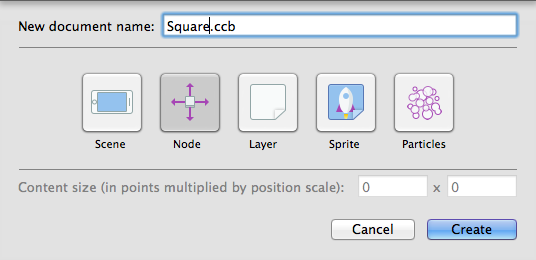
\includegraphics[width=250pt]{images/firstproject/square_ccb.png}
		%\label{labelstruct} 
\end{figure}
The squares we generate in the game shall have a color. A default \ccnode{}
cannot display a color. In order to display a color we need to use a
\inlinecode{CCNodeColor}. The \SB{} node for a CCNodeColor is called
\textit{Color Node}. The root node of every \ccbfile{} is a plain \ccnode{},
that cannot be changed. This means we need to add the \textit{Color Node} as a
child of the root node of \textit{Square.ccb}:
\begin{figure}[H]
		\centering
		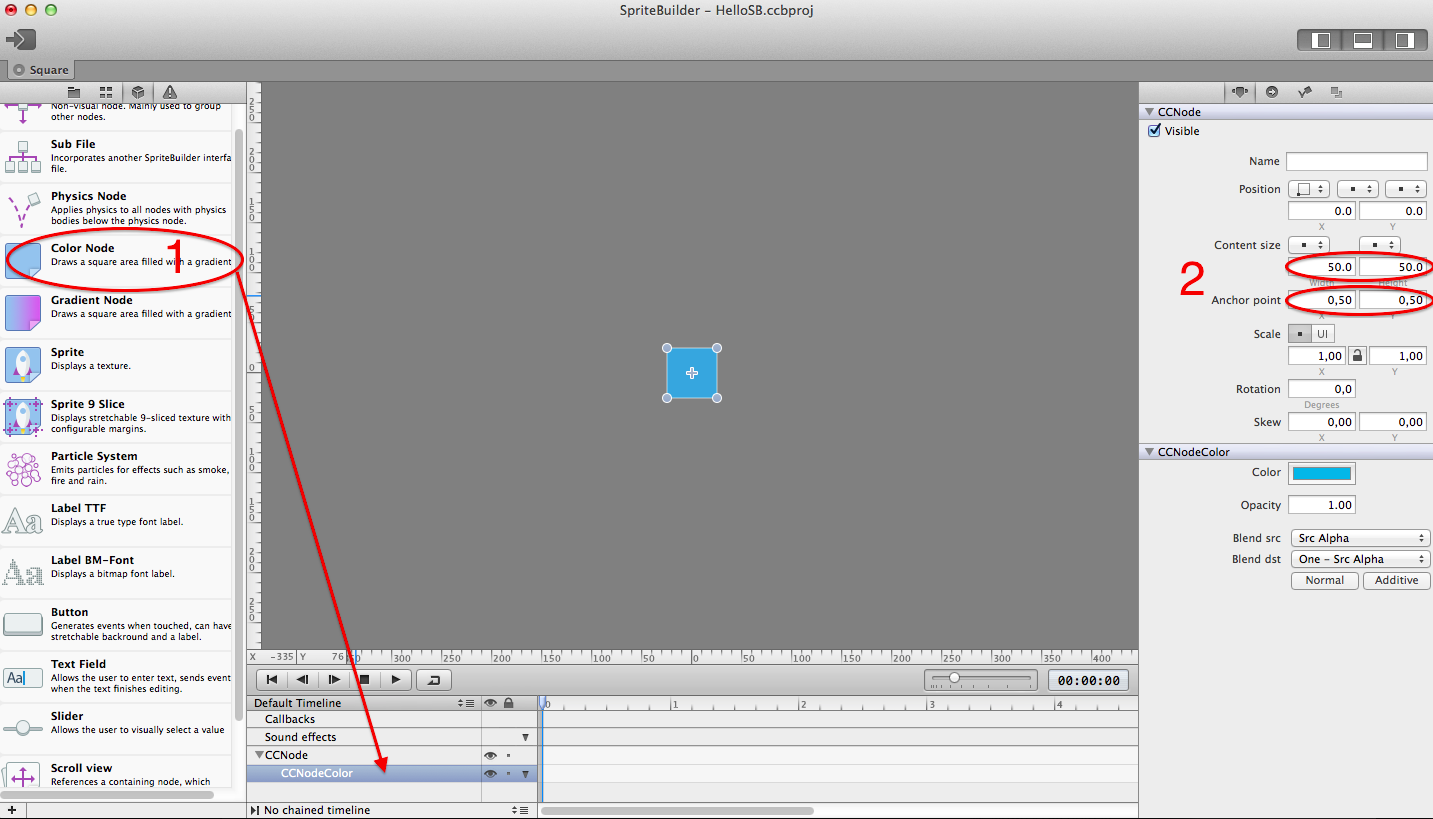
\includegraphics[width=0.9\linewidth]{images/firstproject/square_add_colornode.png}
		%\label{labelstruct} 
\end{figure}
\begin{description}
\item[(1)] Open the \textit{Node Library} and drag a \textit{Color Node} to the
stage or the timeline in order to add it to the root node of of
\textit{Square.ccb}.
\item[(2)] Center the new \textit{Color Node} on the root node by selecting an
\textit{Anchor Point} of (0.5, 0.5). Change the \textit{Content Size} of the
node to (50, 50).
\end{description}

Now the basic square is set up. Next, we need to set up a code connection. Earlier you have seen
the use of \textit{Custom Classes} and \textit{Callbacks}, now we will use the
third type of code connections supported by \SB{} a \textit{Variable
Assignment}.\index{Code Connections!Variable Assignment}. Variable assignments
are generally used when we want to access a part of our scene graph in code. In
our game, whenever a new square is created we want to set a random color for
this square. Generating a random color is something we need to do in code and
cannot do in \SB{}. This also means that we need a way to \textit{apply} the random color we
generate in code to our square that we have set up in \SB{}. The displayed color
is defined in the \textit{Color Node} that we just added. We will need a
reference to this \textit{Color Node} to change the color of our square from
code. \textbf{Select CCNodeColor from the timeline} (and make sure that you
have selected the Color Node and not the Root Node!) and open the connection tab
(the second tab on the right pane):
\begin{figure}[H]
		\centering
		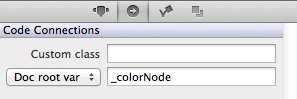
\includegraphics[width=250pt]{images/firstproject/square_code_connection.png}
\end{figure}
As the variable name (entered in the text field), choose \textit{\_colorNode}.
As the second option you need to choose the object to which this variable will be
assigned to. Just as for callbacks you can choose between the \textit{Document
Root} and the \textit{Owner} (\ref{DocumentRoot_Owner}). We choose the
\textit{Document Root}, which means that \SB{} will attempt to store a reference
to the \textit{Color Node} in an instance variable called \textit{\_colorNode}
 on the root node object of this \ccbfile{}. We now face the same 'problem' as earlier when we set up a
\textit{Callback}. The root node of \textit{Square.ccb} is a plain \ccnode{} and
a plain \ccnode{} does not have an instance variable called
\textit{\_colorNode}! We once again need to define a custom class for the root
node of this \ccbfile{}.

\begin{lamp}[frametitle={Variable Assignments, Callbacks and Custom Classes}] 
Always remember that you practically cannot set up a \textit{Variable
assignment} or a \textit{Callback} for the \textit{Document Root} without also
setting a custom class for the root node of the corresponding \ccbfile{}. %TODO:
%flesh out?
\end{lamp}

\textbf{Select the root CCNode node} from the timeline and set the custom class
for this node to \textit{Square}:
\begin{figure}[H]
		\centering
		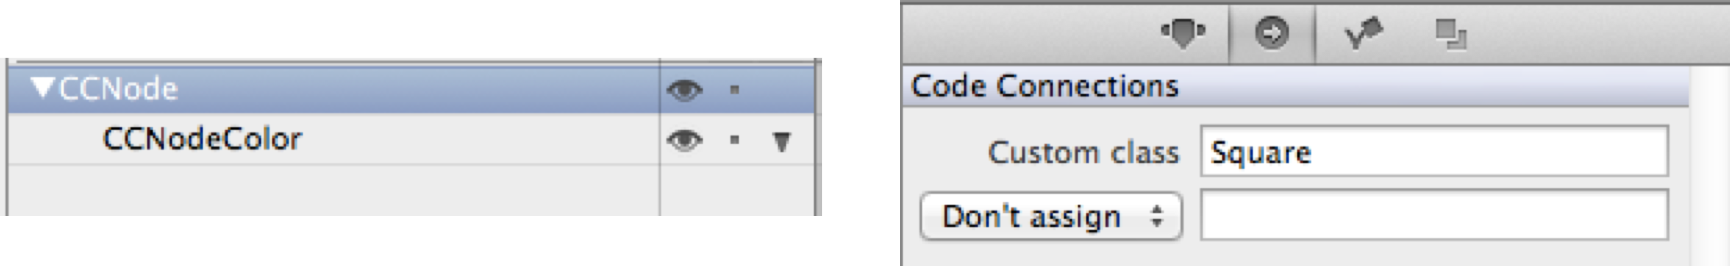
\includegraphics[width=350pt]{images/firstproject/square_custom_class.png}
\end{figure}
When the \textit{CCBReader} reads this \ccbfile{} it will create instance of the
class \textit{Square} as the root node and it will assign a reference to the
\textit{Color Node} to an instance variable of \textit{Square} called
\textit{\_colorNode}. This way we will be able to access the \textit{Color Node}
and change the color of our square programmatically!

\subsubsection{Setting up a custom class for the Gameplay}
In our \textit{Gameplay} scene we want to respond to touches and spawn squares.
All of that functionality needs to be implemented in code. Therefore we need to
define a custom class for the root node of our \textit{Gameplay.ccb} (if you
struggle with the following instructions you can double check how we set up a
custom class for \textit{Square.ccb}).

\begin{enumerate}
  \item Open \textit{Gameplay.ccb}
  \item Select the root \ccnode{} from the timeline
  \item Open the code connections tab (the second tab on the right pane)
  \item Define the \textit{Custom Class} to be \textit{Gameplay}
\end{enumerate}

We've set up multiple code connections throughout this chapter. In order for all
of them to work, we need to \textbf{publish the \SB{} project} and switch to the
\xcode{} project and create the classes and instance variables that we are referencing in the \SB{} project.

\subsubsection{Creating the Square class}
Open \xcode{} and create a new Objective-C class by selecting \textit{File ->
New File\ldots} and choosing \textit{Objective-C class}. As class name choose
\textit{Square} and define it to be a subclass of \ccnode{}. Remember, a custom
class always has to be a subclass of the node type you have selected in \SB{}.
The node type of the root node of \textit{Square.ccb} is a \ccnode{} therefore
\inlinecode{Square} needs to be a subclass of \ccnode{}.

Now open \textit{Square.m} and add the instance variable
\inlinecode{\_colorNode} to the \inlinecode{Square} class. This variable is the
one that we defined in \SB{} to store the reference to the
\inlinecode{CCNodeColor} that displays the color of our square:

\begin{lstlisting}
#import "Square.h"

@implementation Square {
  CCNodeColor *_colorNode;
}

@end
\end{lstlisting} 
After adding the instance variable the code for \textit{Square.m} should look as
shown above. Now that we have a reference to the \inlinecode{CCNodeColor} we
need a position in code where we can set a random color for that node.

The requirements for this projects state that we need to choose a random color
for our Square as soon as it is added to the Gameplay scene. \textbf{How can we
be informed about the square being added to the Gameplay scene?} Therefore we
need to take a closer look at what we call the \textbf{Node
Lifecycle}\index{Node Lifecycle}.

We have five important methods that inform us about certain lifecycle events on
\ccnode{} subclasses. All of the methods below are called on all nodes that are
part of the scene that is being loaded/presented/hidden:

\begin{description}
  \item[didLoadFromCCB] this method is called when the \inlinecode{CCBReader}
  has created the complete node graph from a CCB file and all code connections
  are set up. You implement this method to access and manipulate the content of
  a node. You cannot access child nodes of the node or code connection
  variables before this method is called. Note that this method is only called
  on nodes that are loaded from \ccbfile{}s.
  \item[onEnter/onEnterTransitionDidFinish] are called as soon as a node enters
  the stage. If you are presenting a scene with an animated transition,
  \inlinecode{onEnter} will be called on that scene as soon as the transition
  starts and \inlinecode{onEnterTransitionDidFinish} will be called when the transition
  completes. If a scene or node is being presented/added without an animated
  transition both methods are called directly after each other.
  \item[onExitTransitionDidStart/onExit] are called as soon as a node leaves the
  stage. If you are hiding a scene with an animated transition,
  \inlinecode{onExitTransitionDidStart} will be called on that scene as soon as
  the transition starts and \inlinecode{onExit} will be called when the
  transition completes. If a scene or node is being hidden/removed without an
  animated transition both methods are called directly after each other.
\end{description}

You will get to see lots of examples of how to use the lifecycle methods
throughout this book, for now we know that we need to override
\inlinecode{onEnter} to pick and apply a random color for our square as soon as
it gets added to the Gameplay scene. It is also important to know that you need
to call the \inlinecode{super} implementation if you override any of the 
\inlinecode{onEnter\ldots} or \inlinecode{onExit\ldots} methods. \ccnode{}
has its own implementation of these methods and they are important for the
functionality of the framework - if you do not call them this will result in
unexpected behaviour throughout your game. 
\begin{details}[frametitle={Overriding \cocos{} lifecycle methods}]
As of \cocos{} 3.1 not calling \inlinecode{super} when overriding one of these
lifecycle methods will result in a compiler warning - this can save a lot of
debugging time. You are interested in how that can be done? \cocos{} makes use
of a nice compiler feature to implement this requirement. You simply need to
add an according \inlinecode{\_\_attribute\_\_} to the method definition:

\begin{lstlisting}
 -(void) onEnter __attribute__((objc_requires_super));
\end{lstlisting}

\end{details}
Add this implementation of
\inlinecode{onEnter} to \textit{Square.m}:
\begin{lstlisting}
- (void)onEnter {
  [super onEnter];
  
  // arc4random_uniform(N) generates a random number between 0 and N-1
  float red =   arc4random_uniform(256) / 255.f;
  float green = arc4random_uniform(256) / 255.f;
  float blue =  arc4random_uniform(256) / 255.f;
  
  _colorNode.color = [CCColor colorWithRed:red green:green blue:blue];
}
\end{lstlisting}
The lines above generate three random numbers, one for each color component
with a value between 0.0 and 1.0. These three numbers are used to create an
instance of \inlinecode{CCColor} and set it as the color of our node. 

Now the square will appear in a random color as soon as we add it to a scene.
The second requirement for our square is that it shall rotate while on the
screen. One of the ways to move and/or animate a node in \cocos{} is using the
\cocos{} Action System\index{Action System}. The Action System provides a simple
and expressive way for developers to implement animated changes like:
\textit{Move the main character to the top left corner in 2 seconds}. 

The Action System consists of
dozens of subclasses of \inlinecode{\ccaction{}} - a majority of these actions represent some type of animated movement or
transformation. \inlinecode{CCActionMoveTo} for example moves a node to a
target position within a provided time interval. This is how to use it:
\begin{lstlisting}
CCAction *move = [CCActionMoveTo actionWithDuration:2.f position:ccp(20, 100)];
[aSimpleNode runAction:move];
\end{lstlisting}
All actions can be run by calling the \inlinecode{runAction} method and
providing the action as an argument. 

\begin{details}[frametitle={More about the
\cocos{} Action System}] The \cocos{} Action System is one of the most
important building blocks for most games and we will discuss it in detail
throughout this book. If you want to learn more about the \cocos{} action system
right away, you can check the according chapter in the \cocos{} documentation:
\url{https://www.makegameswith.us/docs/#!/cocos2d/1.0/animations-movements}
\end{details}

The Action System also provides several actions that take other actions as
arguments. One example is \inlinecode{CCActionReverse} that reverses the action
it is initialized with - for example moving a node backwards instead of
forwards. Another example is \inlinecode{CCActionRepeatForever} that takes
another action and - exactly, repeats it forever!

Add the following lines to the \inlinecode{onEnter} method of \textit{Square.m}
to make the square rotate endlessly:
\begin{lstlisting}
CCActionRotateBy *rotate = [CCActionRotateBy actionWithDuration:2.f angle:360.f];
CCActionRepeatForever *repeatRotation = [CCActionRepeatForever actionWithAction:rotate];
[self runAction:repeatRotation];
\end{lstlisting}
One of the nicest aspects of the Action System is that it produces very readable
code, just as the one shown above. We rotate our square by 360 degrees in 2
seconds and repeat that forever!

Finally our implementation of \inlinecode{Square} is complete. Along the way you
have learned about code connections, generating random numbers and using the
action system. Now let's move on to implement the \inlinecode{Gameplay} class so
that we can see our delightfully colored and rotating squares in action.

\subsubsection{Creating the Gameplay class}

After we have set up all the code for the square it's now time to implement the
gameplay. In \SB{} we have already created the \ccbfile{} \textit{Gameplay.ccb}
and set up the custom class for the root node to be \inlinecode{Gameplay}. Now we need to add the
\inlinecode{Gameplay} class in \xcode{} and implement touch handling code that
creates a square and adds it to the gameplay scene as soon as a player touches
the screen.

Create the new class just as you have created the \inlinecode{Square} class. In
\xcode{} select \textit{File -> New -> File\ldots} and select
\textit{Objective-C} class. Again, this class needs to be a subclass of
\ccnode{} since the root node of \textit{Gameplay.ccb} is a \ccnode{}.

\subsubsection{Adding Touch Handling to the
Gameplay}\label{Introduction_FirstTouchHandling} Now we need to add touch
handling to the Gameplay scene. This will be the first time you will add User Interaction to a \cocos{} game! 

The \cocos{} touch handling system works on a \textit{per node
basis}\index{Touch Handling}.
This means that every \ccnode{} instance can choose to receive touches or not. You
can activate touch handling on any node using the
\inlinecode{userInteractionEnabled} property. If
\inlinecode{userInteractionEnabled} is set to \inlinecode{YES}, \cocos{} will
automatically check if your node is touched by the user. In \cocos{} the front
most node receives touch events first.

Each touch in \cocos{} has a lifecycle. That lifecycle consists of four
different states and four corresponding methods that are called on your
\ccnode{}:

\begin{description}
\item[touchBegan:] called when a touch begins
\item[touchMoved:] called when the touch position of a touch changes
\item[touchEnded:] called when a touch ends because the user stops touching the
screen
\item[touchCancelled:] called when a touch is cancelled because user moves touch
outside of the touch area of a node
\end{description}

You can override all of these methods in any \ccnode{} subclass in order to
respond to these lifecycle events. For our simple example now, we only need to
respond to the \inlinecode{touchBegan:} method.

\begin{details}[frametitle={The \cocos{} Touch System}]
We will see more complicated use cases of the \cocos{} touch system throughout
other examples in this book. If you are interested in more details right away
you should
read:\url{https://www.makegameswith.us/docs/#!/cocos2d/1.1/user-interaction} and
\url{https://www.makegameswith.us/gamernews/366/touch-handling-in-cocos2d-30}.
\end{details}

Now that you know the basics, let's implement touch handling for the
\inlinecode{Gameplay} class. First, we need to enable user interaction. A great
place to do this is in the \inlinecode{onEnterTransitionDidFinish} method. Why?
If you have an animated transition that presents your gameplay scene you will
likely not want to the player to interact with your game before this transition
has finished entirely. Add the following method to \textit{Gameplay.m}:
\begin{lstlisting}
- (void)onEnterTransitionDidFinish {
    [super onEnterTransitionDidFinish];
    
    self.userInteractionEnabled = YES;
}
\end{lstlisting}
As discussed earlier you need to call the \inlinecode{super} implementation of
the lifecycle method you are overriding. In the second step we are setting
\inlinecode{userInteractionEnabled} to \inlinecode{YES}. Now \cocos{} knows that
this node wants to receive touch events. 

In the next step we need to decide to which touch events we
want to subscribe and implement the corresponding method. For this simple game
we only need to know when a touch begins, because we will add a square to the
screen immediately. This means we only need to implement the
\inlinecode{touchBegan:} method. Add the following implementation to
\inlinecode{Gameplay.m}:
\begin{lstlisting}
- (void)touchBegan:(UITouch *)touch withEvent:(UIEvent *)event {
    CGPoint touchPosition = [touch locationInNode:self];
    CCNode *square = [CCBReader load:@"Square"];
    [self addChild:square];
    square.position = touchPosition;
}
\end{lstlisting}
We have now implemented the \inlinecode{touchBegan:} method. It will be called
every time the user taps onto the gameplay scene. As one parameter of this
method we receive a \inlinecode{UITouch}. The \inlinecode{UITouch} stores all
information about the touch. \cocos{} adds a method called
\inlinecode{locationInNode:}. This method returns the touch position
relative to the provided node. In the first line we call this method to receive
the touch location within the gameplay scene (referred to by \inlinecode{self}).
In the next line we load one \inlinecode{Square} node using the
\inlinecode{CCBReader}. Then we add that loaded square as a child to the
gameplay scene. The \inlinecode{addChild:} method of \ccnode{} will add the
square to the node hierarchy of the gameplay scene. As soon as node becomes part
of the node hierarchy of the currently active scene it will be displayed on the
screen. Finally we choose a position for the square.
We provide the touch position that we determined in the first line - this way the square will be spawned exactly at the position touched by
the player. Now it's time to run your project again. Once the game started,
select the \textit{Start} button to go to the gameplay scene then click onto the
screen multiple times to simulate touches. Every time you simulate a touch you
should see a new square spawn at the touch position:
\begin{figure}[H]
		\centering
		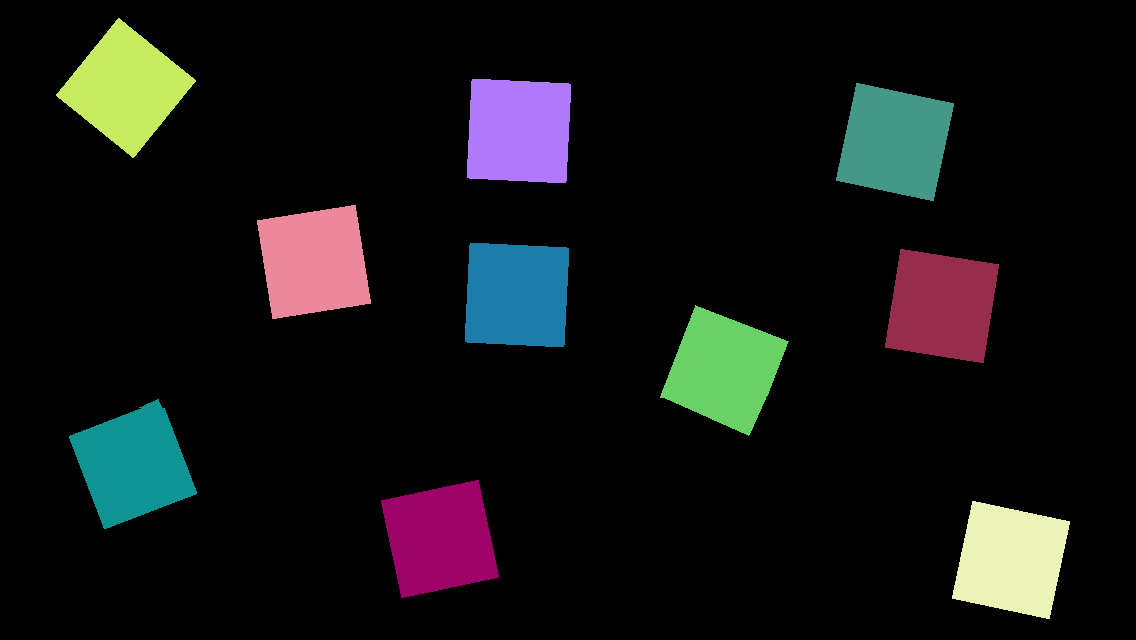
\includegraphics[width=350pt]{images/firstproject/spinning_squares.png}
\end{figure}
\textbf{Well done!} You have come a very long way from the blank project to a
first simple game that uses scene transitions, actions and the \cocos{} touch
system. But this is only the very beginning. In the next chapter we will start
working on a much more complex game that will teach you many more important
concepts of \SB{} and \cocos{}. 

\section{Exercises}
Now it's time for some exercises. Note that you can't find all the knowledge
for these exercises in this chapter - for some exercise you may will have to use
the help of the internet (that is another exercise right there).
\begin{description}
\item[1.0] Add a label to the top right corner of the gameplay scene. This label
shall display the amount of squares that are currently on the screen.
\item[1.1] Make each square disappear after it has been on the screen for 2
seconds. 
\end{description}
